\documentclass[11pt,a4paper]{article}

% ── Packages ──
\usepackage[utf8]{inputenc}
\usepackage[T1]{fontenc}
\usepackage{fontspec}
\setmainfont{Liberation Sans}
\usepackage[margin=2.5cm]{geometry}
\usepackage{graphicx}
\usepackage{booktabs}
\usepackage{tabularx}
\usepackage{multirow}
\usepackage{caption}
\usepackage{subcaption}
\usepackage{hyperref}
\usepackage{xcolor}
\usepackage{amsmath,amssymb}
\usepackage{natbib}
\usepackage{longtable}
\usepackage{array}
\usepackage{float}
\usepackage{enumitem}

\hypersetup{colorlinks=true, linkcolor=blue, citecolor=blue, urlcolor=blue}

% ── Title ──
\title{Mineral-Pathway Transcriptional and Molecular Responses to Spaceflight: \\
       A Multi-Omics Analysis of Astronaut and Rodent Data from the NASA OSDR}
\author{Richard Barker}
\date{}

\begin{document}

\maketitle

% ════════════════════════════════════════════════════════════════════
% ABSTRACT
% ════════════════════════════════════════════════════════════════════
\begin{abstract}
\noindent
Spaceflight induces physiological stressors including microgravity, radiation, and altered fluid shifts that may disrupt mineral homeostasis. We mined the NASA Open Science Data Repository (OSDR) to identify evidence of mineral deficiencies linked to transcriptional and molecular responses in astronauts and rodents. Multi-omics data from the Inspiration4 (I4) mission (4 civilian astronauts, 3-day low-Earth orbit, September 2021) including RNA-seq, proteomics, metabolomics, and clinical chemistry panels (CMP, CBC) were integrated with rodent liver RNA-seq from Rodent Research missions (OSD-47). We constructed mineral-pathway gene sets spanning 10 minerals (Ca, Fe, Mg, Zn, Cu, Se, K, Na, P, Mn) from KEGG pathways and curated literature, yielding 352 validated mineral homeostasis genes and 585 KEGG pathway genes. Cross-referencing astronaut differential expression results identified 46 significant mineral-pathway genes (|log$_2$FC| $>$ 0.5, $p$ $<$ 0.05), including copper-dependent enzymes (APP up, LOX/LOXL1 down), magnesium-binding S100 proteins (S100A8/A9/A12 down), and the calcium channel CACNA1D (down, log$_2$FC = $-$2.14). Machine learning regression demonstrated that mineral-pathway gene expression predicts serum potassium ($r$ = 0.50, $R^2$ = 0.12) and sodium ($r$ = 0.46, $R^2$ = 0.19) levels under leave-one-out cross-validation. Permutation importance identified CAMK4, SLC30A7, SELENOW, SLC11A1, and ALPL as top predictive genes. Cross-species concordance analysis between astronaut peripheral blood and rodent liver revealed no significant directional concordance (Spearman $r$ = 0.007, $p$ = 0.87), suggesting tissue- and mission-duration-specific mineral-pathway responses. These findings provide transcriptomic and proteomic evidence that spaceflight alters mineral homeostasis pathways, with implications for countermeasure development and nutritional monitoring during long-duration spaceflight.

\medskip
\noindent\textbf{Keywords:} spaceflight, mineral deficiency, multi-omics, transcriptomics, proteomics, KEGG pathways, NASA OSDR, Inspiration4, cross-species concordance, machine learning
\end{abstract}

% ════════════════════════════════════════════════════════════════════
% INTRODUCTION
% ════════════════════════════════════════════════════════════════════
\section{Introduction}

Spaceflight exposes humans to a unique combination of physiological stressors including microgravity, cosmic radiation, confinement, and altered circadian rhythms. These stressors affect multiple biological systems, including bone metabolism, cardiovascular function, immune response, and nutritional status \citep{williams2009}. Mineral homeostasis is particularly vulnerable during spaceflight: microgravity-induced bone loss releases calcium into the circulation \citep{smith2005}, fluid shifts expand central blood volume \citep{norsk2015}, and spaceflight increases oxidative stress \citep{stein2002}.

The NASA Open Science Data Repository (OSDR) provides open access to multi-omics data from spaceflight experiments, including the Inspiration4 (I4) mission --- the first all-civilian orbital spaceflight (September 2021, 3-day low-Earth orbit) \citep{overbey2024}. The I4 dataset includes RNA-seq, proteomics, metabolomics, and clinical chemistry from four civilian astronauts across seven timepoints, offering a unique opportunity to study acute mineral-pathway responses to short-duration spaceflight.

Mineral deficiencies are a documented concern in spaceflight medicine. Calcium loss from bone resorption has been observed in astronauts on the International Space Station (ISS) \citep{smith2015}. Iron availability and stores increase during long-duration flight, alongside a loss of red cell mass \citep{smith2002iron}. Zinc and selenium status may be compromised by altered dietary intake and by the post-flight increase in oxidative stress \citep{stein2002}. However, the transcriptional and molecular signatures of these mineral perturbations have not been systematically characterized using multi-omics data.

In this study, we mined astronaut and rodent multi-omics data from the NASA OSDR to: (1) construct comprehensive mineral-pathway gene sets from KEGG pathways and curated literature; (2) identify mineral-pathway genes differentially expressed in response to spaceflight; (3) evaluate whether mineral-pathway gene expression predicts serum mineral levels using machine learning; (4) assess cross-species concordance between astronaut and rodent mineral-pathway responses; and (5) build a systems biology atlas integrating these findings.

% ════════════════════════════════════════════════════════════════════
% METHODS
% ════════════════════════════════════════════════════════════════════
\section{Methods}

\subsection{Data Acquisition}

Astronaut data were retrieved from the NASA OSDR REST API (\texttt{https://visualization.osdr.nasa.gov/biodata/api}). The following studies were downloaded: OSD-569 (RNA-seq gene expression), OSD-570 (snRNA-seq/snATAC-seq), OSD-571 (proteomics and metabolomics DE), OSD-572 (metagenomics), OSD-575 (Comprehensive Metabolic Panel and cytokine panels), OSD-630 (stool metagenomics), and OSD-656 (urine immune panel). All data correspond to the Inspiration4 mission with four civilian astronauts (C001--C004) sampled at seven timepoints: L-92, L-44, L-3 (pre-flight), R+1, R+45, R+82, R+194 (post-flight).

Rodent data were retrieved from OSD-47 (Rodent Research-1, mouse liver RNA-seq, C57BL/6T strain) with three experimental groups: basal (BSL, $n=3$), flight (FLT, $n=3$), and ground control (GC, $n=3$). Normalized gene count matrices were used for differential expression analysis.

\subsection{Mineral-Pathway Gene Set Construction}

We compiled curated mineral homeostasis gene sets for 10 minerals (calcium, iron, magnesium, zinc, copper, selenium, potassium, sodium, phosphorus, manganese) from KEGG pathway hsa04978 (Mineral absorption), UniProt, HGNC, and published literature. Gene symbols were validated against the KEGG human gene database (19,976 genes). Five KEGG pathways relevant to mineral metabolism were included: hsa04978 (Mineral absorption, 61 genes), hsa04020 (Calcium signaling, 254 genes), hsa04216 (Ferroptosis, 42 genes), hsa00190 (Oxidative phosphorylation, 138 genes), and hsa04976 (Bile secretion, 90 genes). The final gene set comprised 801 unique genes, with 97 genes present in both mineral and KEGG pathway sets.

\subsection{RNA-seq Differential Expression Analysis}

The I4 RNA-seq data included two differential expression methods: DESeq2 and a pipeline-transcriptome-de approach. Three flight comparisons were analyzed: I4-FP1 (R+1 vs pre-flight), I4-FP2 (R+1/R+45/R+82 vs pre-flight), and I4-FP3 (R+1/R+45/R+82/R+194 vs pre-flight). The pipeline-transcriptome-de method yielded meaningful fold changes (range $-$2.91 to 2.39) and was used as the primary DE method, as DESeq2 log$_2$FC values were uniformly near zero. ENSEMBL gene IDs were mapped to HGNC symbols via the mygene.info API (73.6\% mapping rate, 45,550 of 61,852 genes).

\subsection{Proteomics and Metabolomics}

Proteomics DE was performed using limma (I4-FP1 and I4-FP2 comparisons) with 3,285 proteins. Metabolomics DE included 2,624 metabolites across two comparisons. Proteomics data already contained gene symbols; metabolomics data used metabolite identifiers.

\subsection{Machine Learning Analysis}

Feature matrices were constructed from RNA-seq count data restricted to mineral-pathway genes (784 genes after aggregating duplicate symbols). Top 200 genes by variance were selected. Two ML tasks were performed:

\textbf{Classification} (flight vs ground): Five classifiers (RandomForest, SVM-RBF, SVM-Linear, LogisticRegression, GradientBoosting) were evaluated with leave-one-out cross-validation (LOO-CV, $n=16$: 4 flight, 12 ground). Balanced class weights were used to address imbalance.

\textbf{Regression} (mineral level prediction): Four regressors (Ridge, SVR-Linear, SVR-RBF, RandomForest) predicted serum calcium, potassium, sodium, and hemoglobin (iron proxy) from gene expression under LOO-CV. Permutation importance (20 repeats) identified key predictive genes.

\subsection{Cross-Species Concordance}

Mouse liver RNA-seq (OSD-47, FLT vs GC) was analyzed using Welch's t-tests with Benjamini-Hochberg correction. Mouse ENSEMBL IDs were mapped to human gene symbols via mygene.info homologene data (13,825 genes mapped). Directional concordance was assessed for 587 shared mineral-pathway genes using Spearman correlation and binomial tests.

\subsection{Systems Biology Atlas}

A composite systems biology atlas was constructed integrating KEGG pathway expression changes, mineral-gene counts, DE gene summaries, cross-species concordance, and top mineral-pathway DE genes into a multi-panel figure.

\subsection{Reproducibility}

All analysis scripts are available in the FAIR-compliant Zenodo package, including pipeline code, processed data, figures, and a data dictionary. Python 3.11 with pandas, scikit-learn, matplotlib, seaborn, and networkx was used for analysis. R 4.4.3 with circlize and ggplot2 was used for supplementary visualizations.

% ════════════════════════════════════════════════════════════════════
% RESULTS
% ════════════════════════════════════════════════════════════════════
\section{Results}

\subsection{Serum Mineral Measurements in I4 Astronauts}

The Comprehensive Metabolic Panel directly measured five minerals across four astronauts at seven timepoints: calcium (9.2--10.3 mg/dL), potassium (3.0--4.6 mmol/L), sodium (137--143 mmol/L), chloride (99--106 mmol/L), and CO$_2$ (23--29 mmol/L). Hemoglobin from the CBC served as an iron status proxy (11.5--17.0 g/dL). Notably, potassium showed a consistent post-flight decline in three of four astronauts (C002: 3.9 $\rightarrow$ 3.5; C003: 3.7 $\rightarrow$ 3.0; C004: 4.2 $\rightarrow$ 4.0 mmol/L at R+1 vs L-92), while calcium remained relatively stable (Figure~\ref{fig:trajectories}).

\begin{figure}[H]
\centering
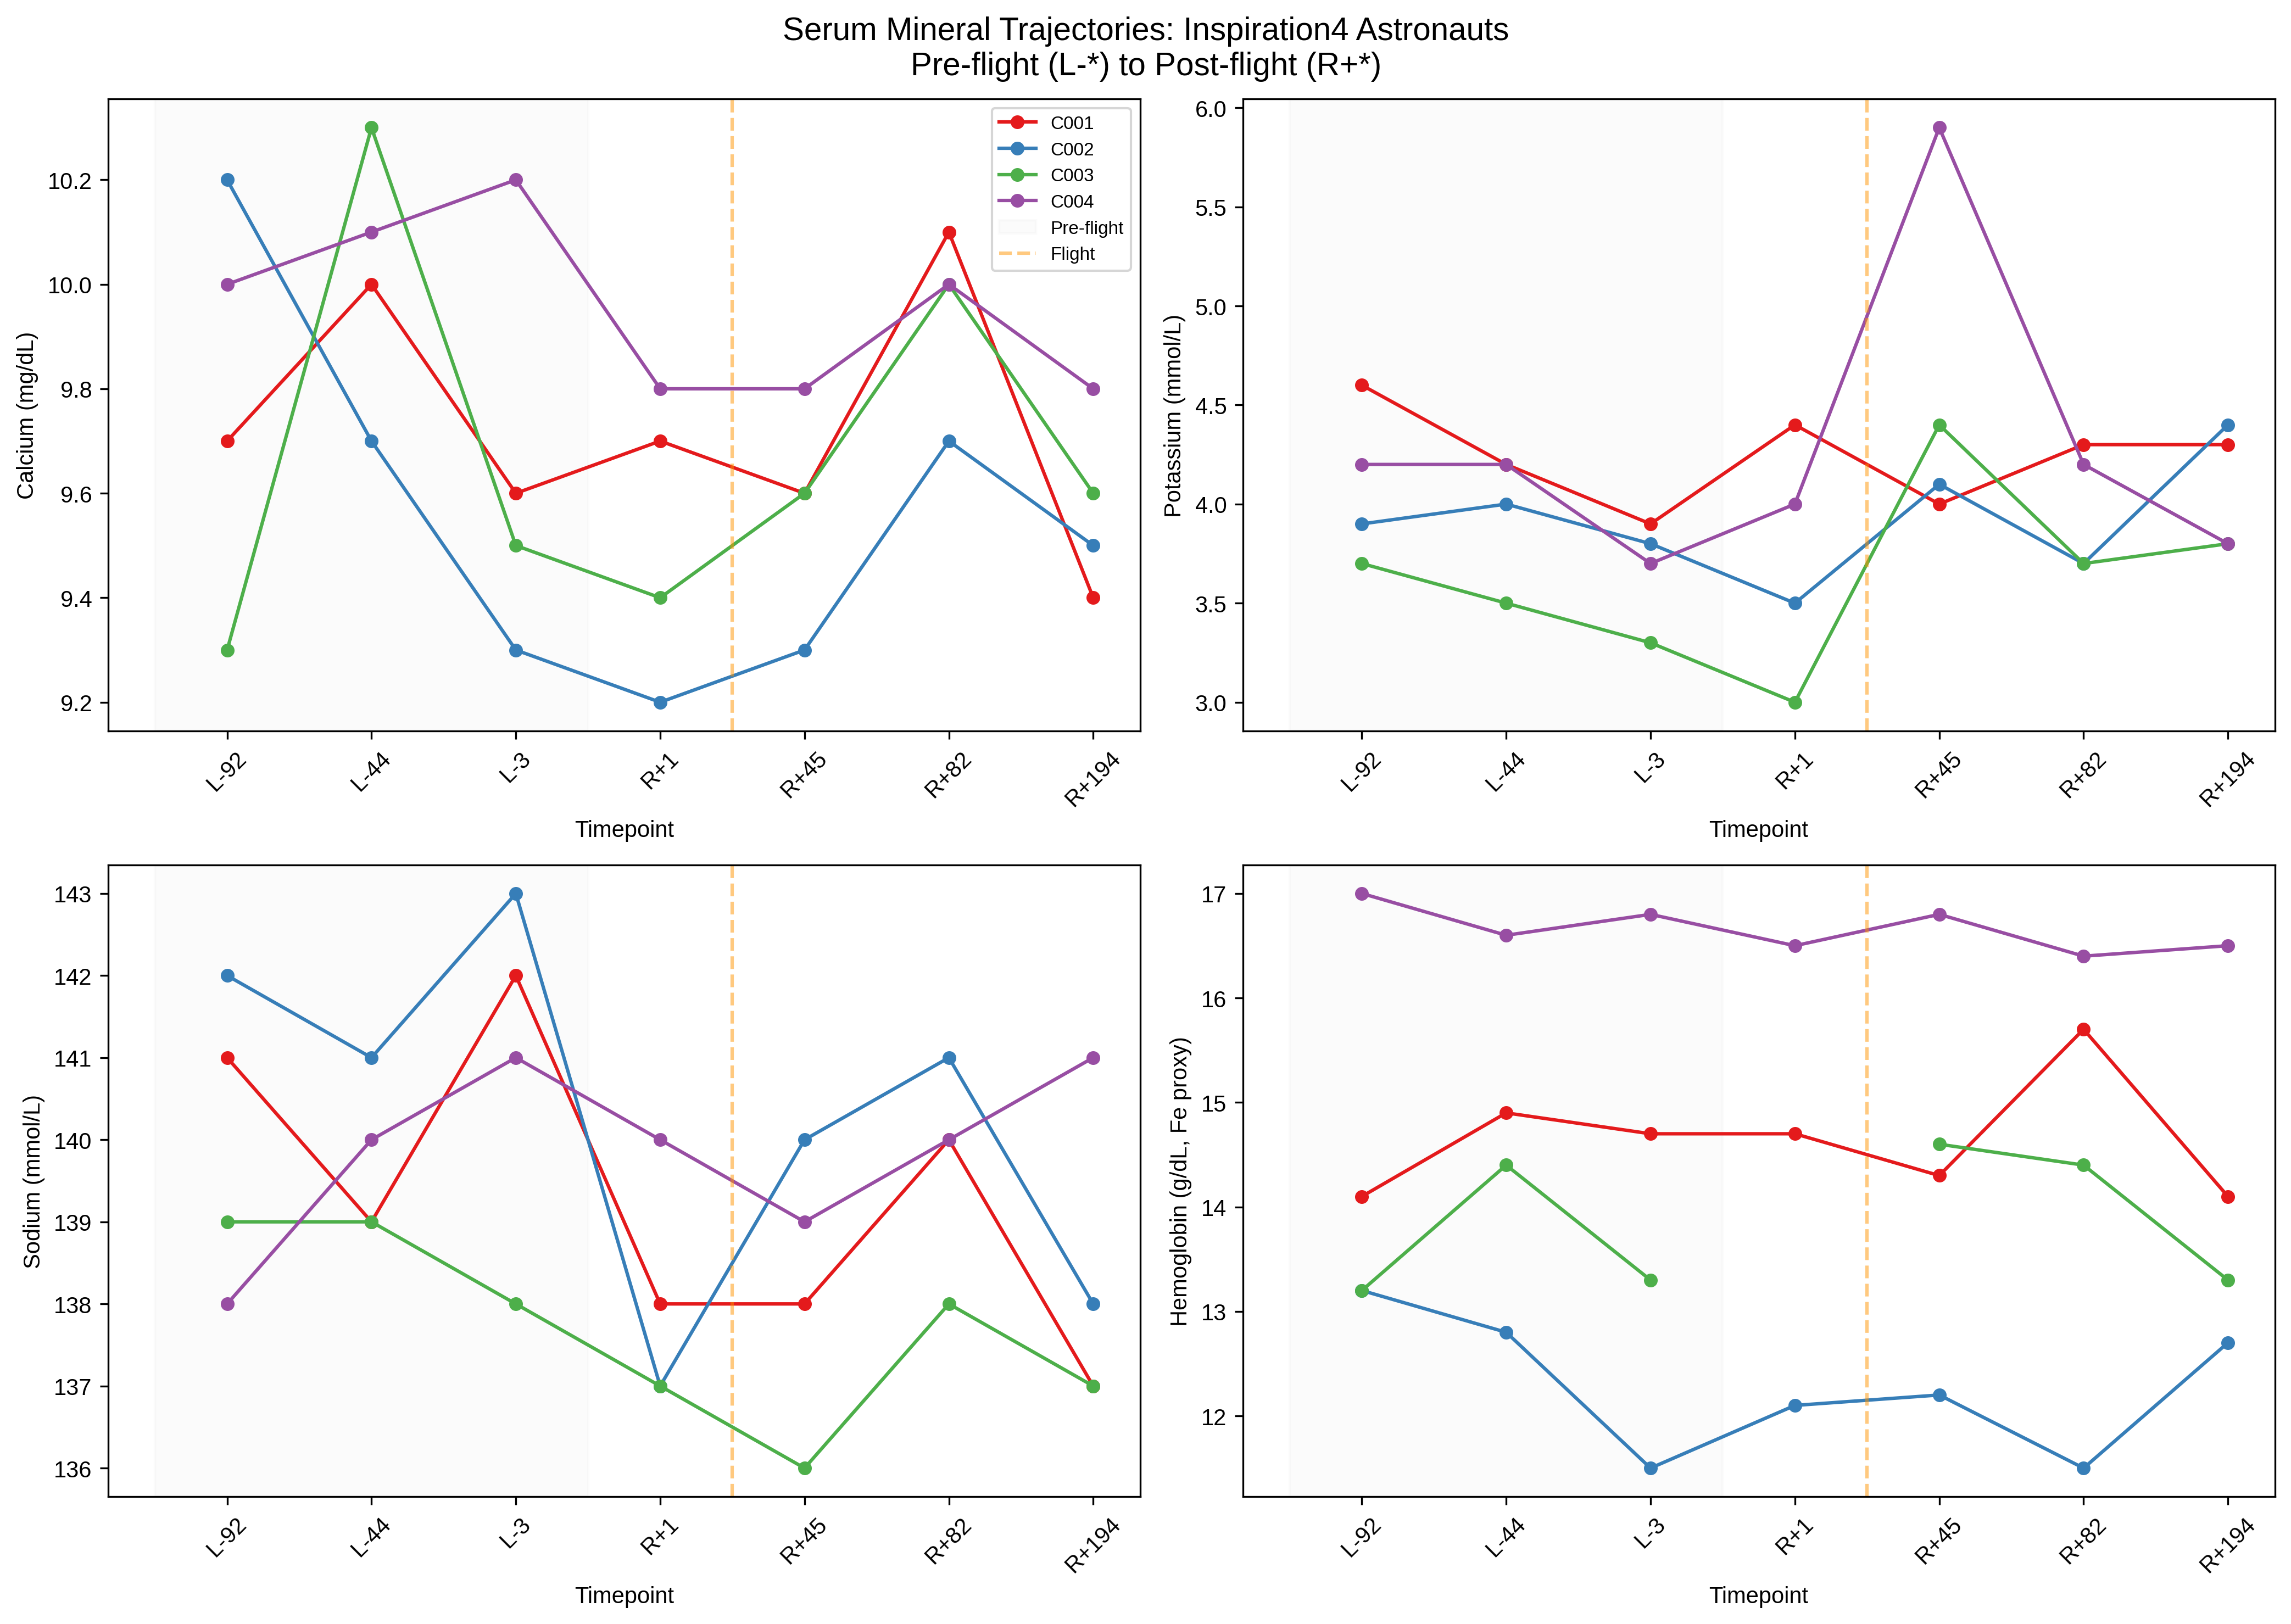
\includegraphics[width=\textwidth]{figures/fig7_mineral_trajectories.png}
\caption{Serum mineral trajectories for Inspiration4 astronauts. Pre-flight timepoints (L-92, L-44, L-3) shown left of the dashed line; post-flight timepoints (R+1, R+45, R+82, R+194) right. Each line represents one astronaut (C001--C004). Potassium shows a consistent post-flight decline in three of four astronauts.}
\label{fig:trajectories}
\end{figure}

\subsection{Mineral-Pathway Gene Set Construction}

We constructed comprehensive mineral-pathway gene sets comprising 352 curated mineral homeostasis genes (validated against KEGG) and 585 KEGG pathway genes across five pathways, totaling 801 unique genes. Eight genes were associated with more than one mineral, and 97 genes were present in both mineral and KEGG pathway sets (Table~\ref{tab:genesets}).

\begin{table}[H]
\centering
\caption{Mineral-pathway gene set summary}
\label{tab:genesets}
\begin{tabular}{lr}
\toprule
\textbf{Gene Set} & \textbf{Gene Count} \\
\midrule
Calcium (curated) & 71 \\
Potassium (curated) & 63 \\
Sodium (curated) & 42 \\
Iron (curated) & 39 \\
Zinc (curated) & 35 \\
Selenium (curated) & 27 \\
Magnesium (curated) & 29 \\
Phosphorus (curated) & 25 \\
Copper (curated) & 24 \\
Manganese (curated) & 3 \\
\midrule
KEGG Calcium signaling (hsa04020) & 254 \\
KEGG Oxidative phosphorylation (hsa00190) & 138 \\
KEGG Bile secretion (hsa04976) & 90 \\
KEGG Mineral absorption (hsa04978) & 61 \\
KEGG Ferroptosis (hsa04216) & 42 \\
\midrule
\textbf{Total unique genes} & \textbf{801} \\
\textbf{Genes in $>$1 mineral} & 8 \\
\textbf{Genes in mineral + KEGG} & 97 \\
\bottomrule
\end{tabular}
\end{table}

\subsection{Mineral-Pathway Differential Expression}

Cross-referencing astronaut DE results with mineral-pathway gene sets identified 46 significant mineral-pathway genes (|log$_2$FC| $>$ 0.5, $p$ $<$ 0.05) across RNA-seq and proteomics (Figure~\ref{fig:heatmap}).

\textbf{RNA-seq} (pipeline-transcriptome-de method): I4-FP1 yielded 20 significant mineral-pathway genes, I4-FP2 yielded 10, and I4-FP3 yielded 16. The most notable findings in I4-FP3 (full follow-up) included:
\begin{itemize}[nosep]
\item \textit{CACNA1D} (calcium channel, log$_2$FC = $-$2.14, $p$ = 0.004) --- down-regulation of a voltage-gated calcium channel
\item \textit{LOXL2} (copper-dependent enzyme, log$_2$FC = +2.10, $p$ = 0.006) --- up-regulation of a lysyl oxidase homolog
\item \textit{VEGFA} (log$_2$FC = $-$1.69, $p$ = 0.007) --- down-regulation of vascular endothelial growth factor
\item \textit{KCNQ2} (potassium channel, log$_2$FC = +1.47, $p$ = 0.037) --- up-regulation of a potassium channel
\item \textit{CNNM1} (magnesium transporter, log$_2$FC = $-$1.46, $p$ = 0.037) --- down-regulation of a magnesium transporter
\end{itemize}

\textbf{Proteomics}: I4-FP1 yielded 12 and I4-FP2 yielded 13 significant mineral-pathway proteins. Key findings included:
\begin{itemize}[nosep]
\item \textit{APP} (copper-related, log$_2$FC = +1.32, $p$ = 3$\times$10$^{-6}$) --- up-regulation of amyloid precursor protein
\item \textit{FXYD2} (sodium pump regulator, log$_2$FC = $-$0.93, $p$ = 6$\times$10$^{-4}$) --- down-regulation of Na/K ATPase subunit
\item \textit{LOX} (copper-dependent enzyme, log$_2$FC = $-$0.72, $p$ = 0.003) --- down-regulation of lysyl oxidase
\item \textit{S100A8/A9/A12} (magnesium-binding, log$_2$FC = $-$0.52 to $-$1.20) --- consistent suppression of S100 proteins
\end{itemize}

\begin{figure}[H]
\centering
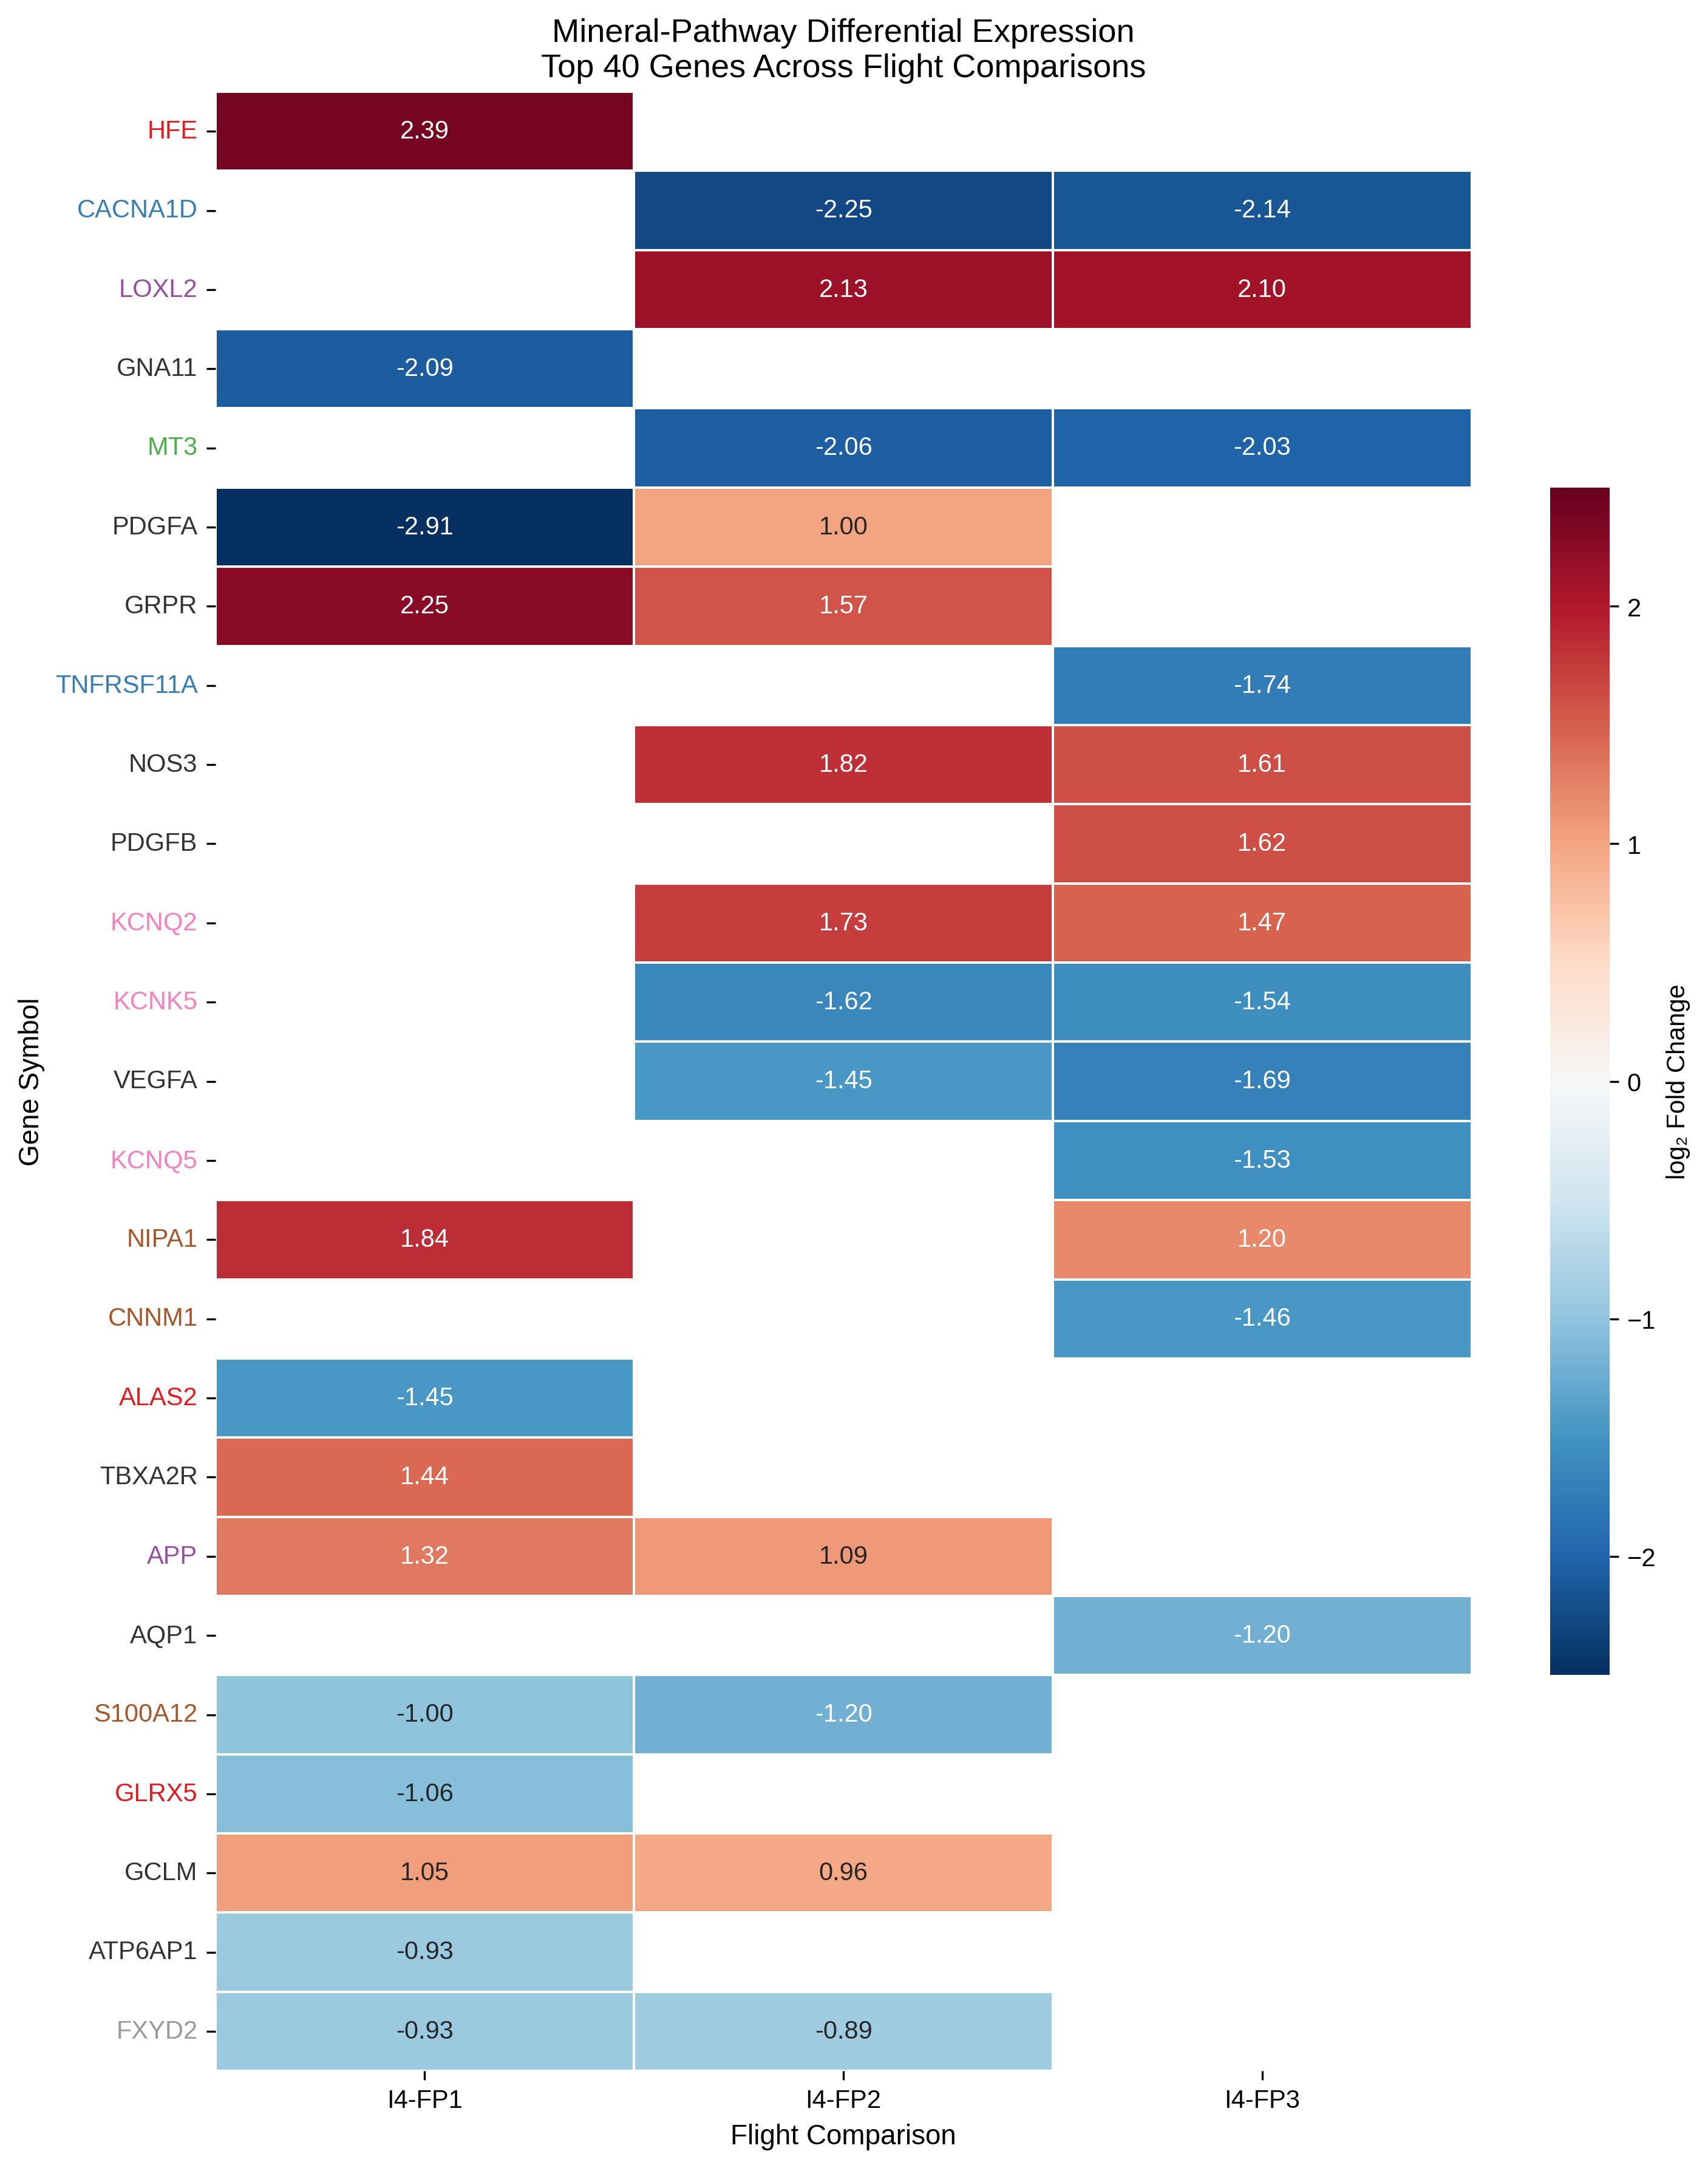
\includegraphics[width=0.85\textwidth]{figures/fig1_heatmap_mineral_de.png}
\caption{Heatmap of the top 40 mineral-pathway differentially expressed genes across three flight comparisons (I4-FP1, I4-FP2, I4-FP3) from RNA-seq and proteomics. Gene labels are colored by their primary mineral association. Red indicates up-regulation; blue indicates down-regulation.}
\label{fig:heatmap}
\end{figure}

\begin{figure}[H]
\centering
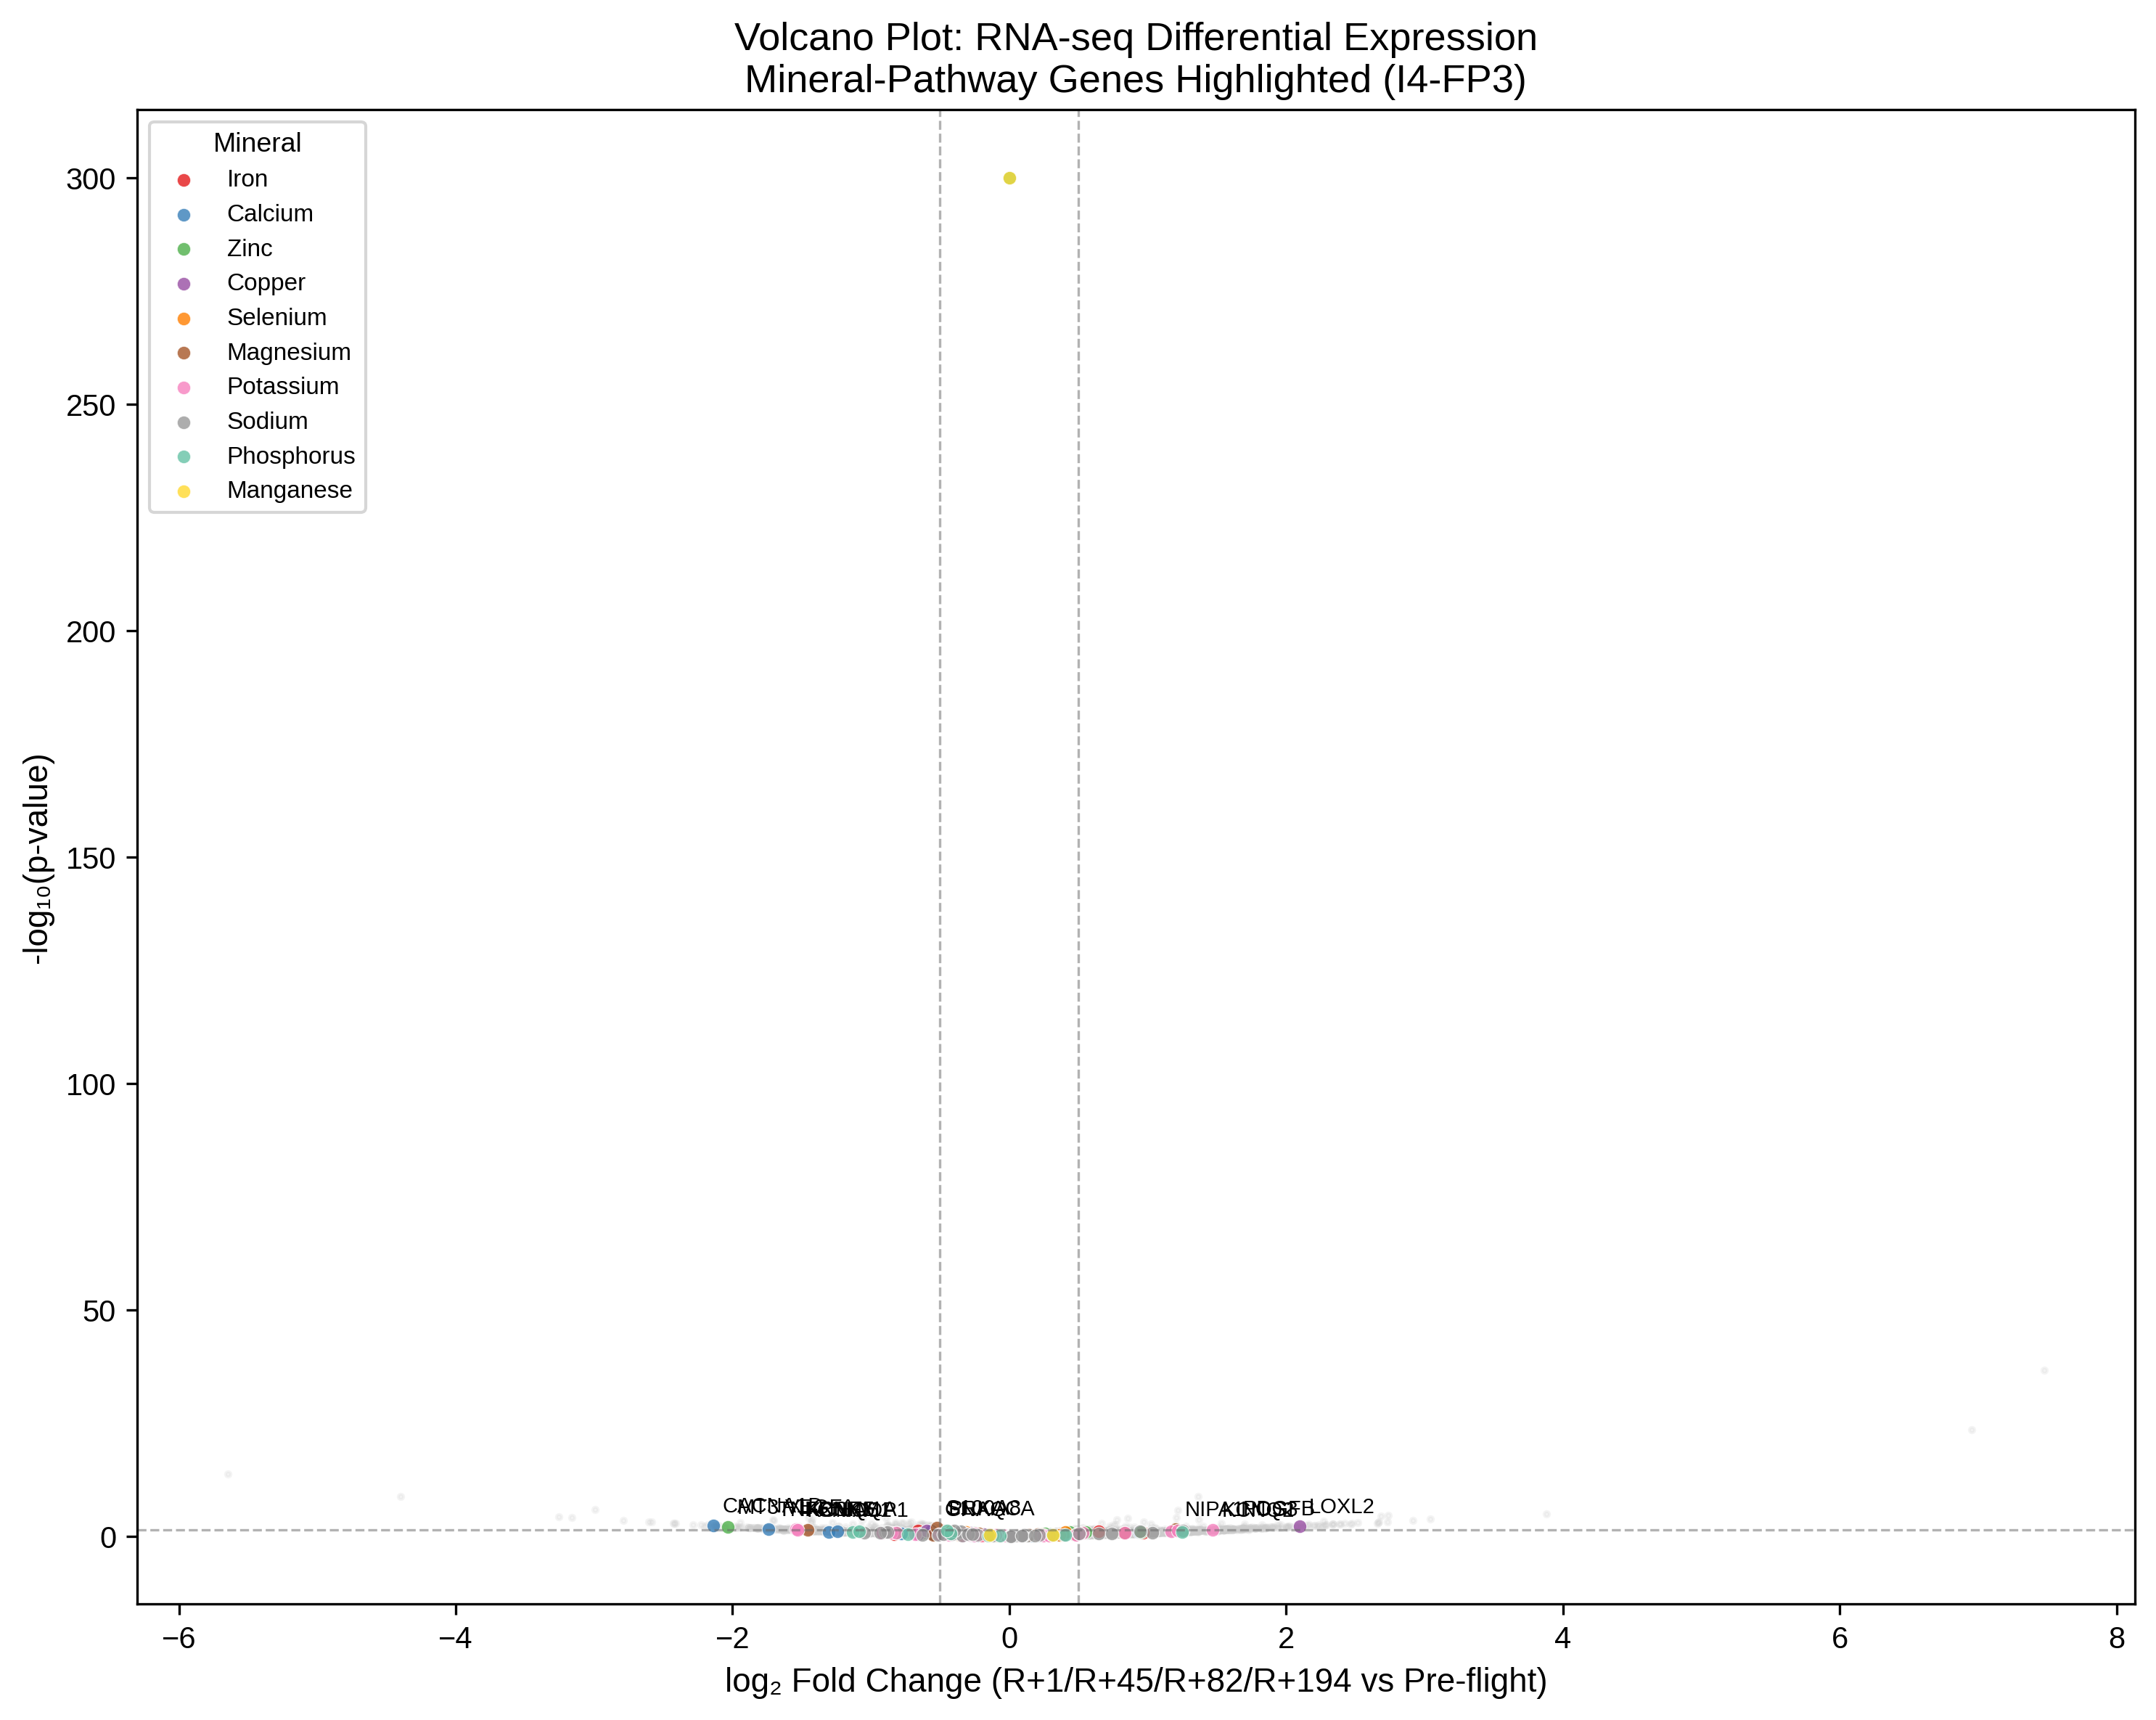
\includegraphics[width=0.9\textwidth]{figures/fig2_volcano_rnaseq.png}
\caption{Volcano plot of RNA-seq differential expression (I4-FP3 comparison). Mineral-pathway genes are highlighted by mineral association. Dashed lines indicate significance thresholds (|log$_2$FC| $>$ 0.5, $p$ $<$ 0.05). Significant mineral-pathway genes are labeled.}
\label{fig:volcano}
\end{figure}

\subsection{Machine Learning: Mineral Level Prediction}

\subsubsection{Classification: Flight vs Ground}

Five classifiers were evaluated under LOO-CV ($n=16$). With balanced class weights, SVM-RBF achieved the highest AUC-ROC of 0.604, though all models struggled with the extreme class imbalance (4 flight vs 12 ground samples). The classification task was limited by the small sample size and the fact that only one post-flight timepoint (R+1) had omics data.

\subsubsection{Regression: Serum Mineral Levels}

Four regressors predicted serum mineral levels from mineral-pathway gene expression under LOO-CV (Table~\ref{tab:regression}). Potassium and sodium regression showed meaningful predictive signal:

\begin{table}[H]
\centering
\caption{Mineral level regression results (best model per target, LOO-CV)}
\label{tab:regression}
\begin{tabular}{llrrr}
\toprule
\textbf{Target} & \textbf{Best Model} & \textbf{$r$} & \textbf{$R^2$} & \textbf{RMSE} \\
\midrule
Potassium & Ridge & 0.500 & 0.122 & 0.377 \\
Sodium & SVR-Linear & 0.460 & 0.193 & 1.611 \\
Hemoglobin (Fe proxy) & SVR-Linear & 0.477 & $-$0.615 & 2.087 \\
Calcium & Ridge & $-$0.015 & $-$0.592 & 0.433 \\
\bottomrule
\end{tabular}
\end{table}

\subsubsection{Permutation Importance}

Permutation importance analysis identified key genes driving mineral level predictions (Figure~\ref{fig:importance}). For potassium regression, top genes included \textit{CAMK4} (calcium signaling), \textit{SLC30A7} (zinc transporter), \textit{SELENOW} (selenium protein), \textit{SLC11A1} (iron transporter), and \textit{ALPL} (calcium/phosphorus). For sodium regression, top genes included \textit{CAMK4}, \textit{ITPKB}, \textit{SLC2A1}, and \textit{PPP3R1} (calcium signaling).

\begin{figure}[H]
\centering
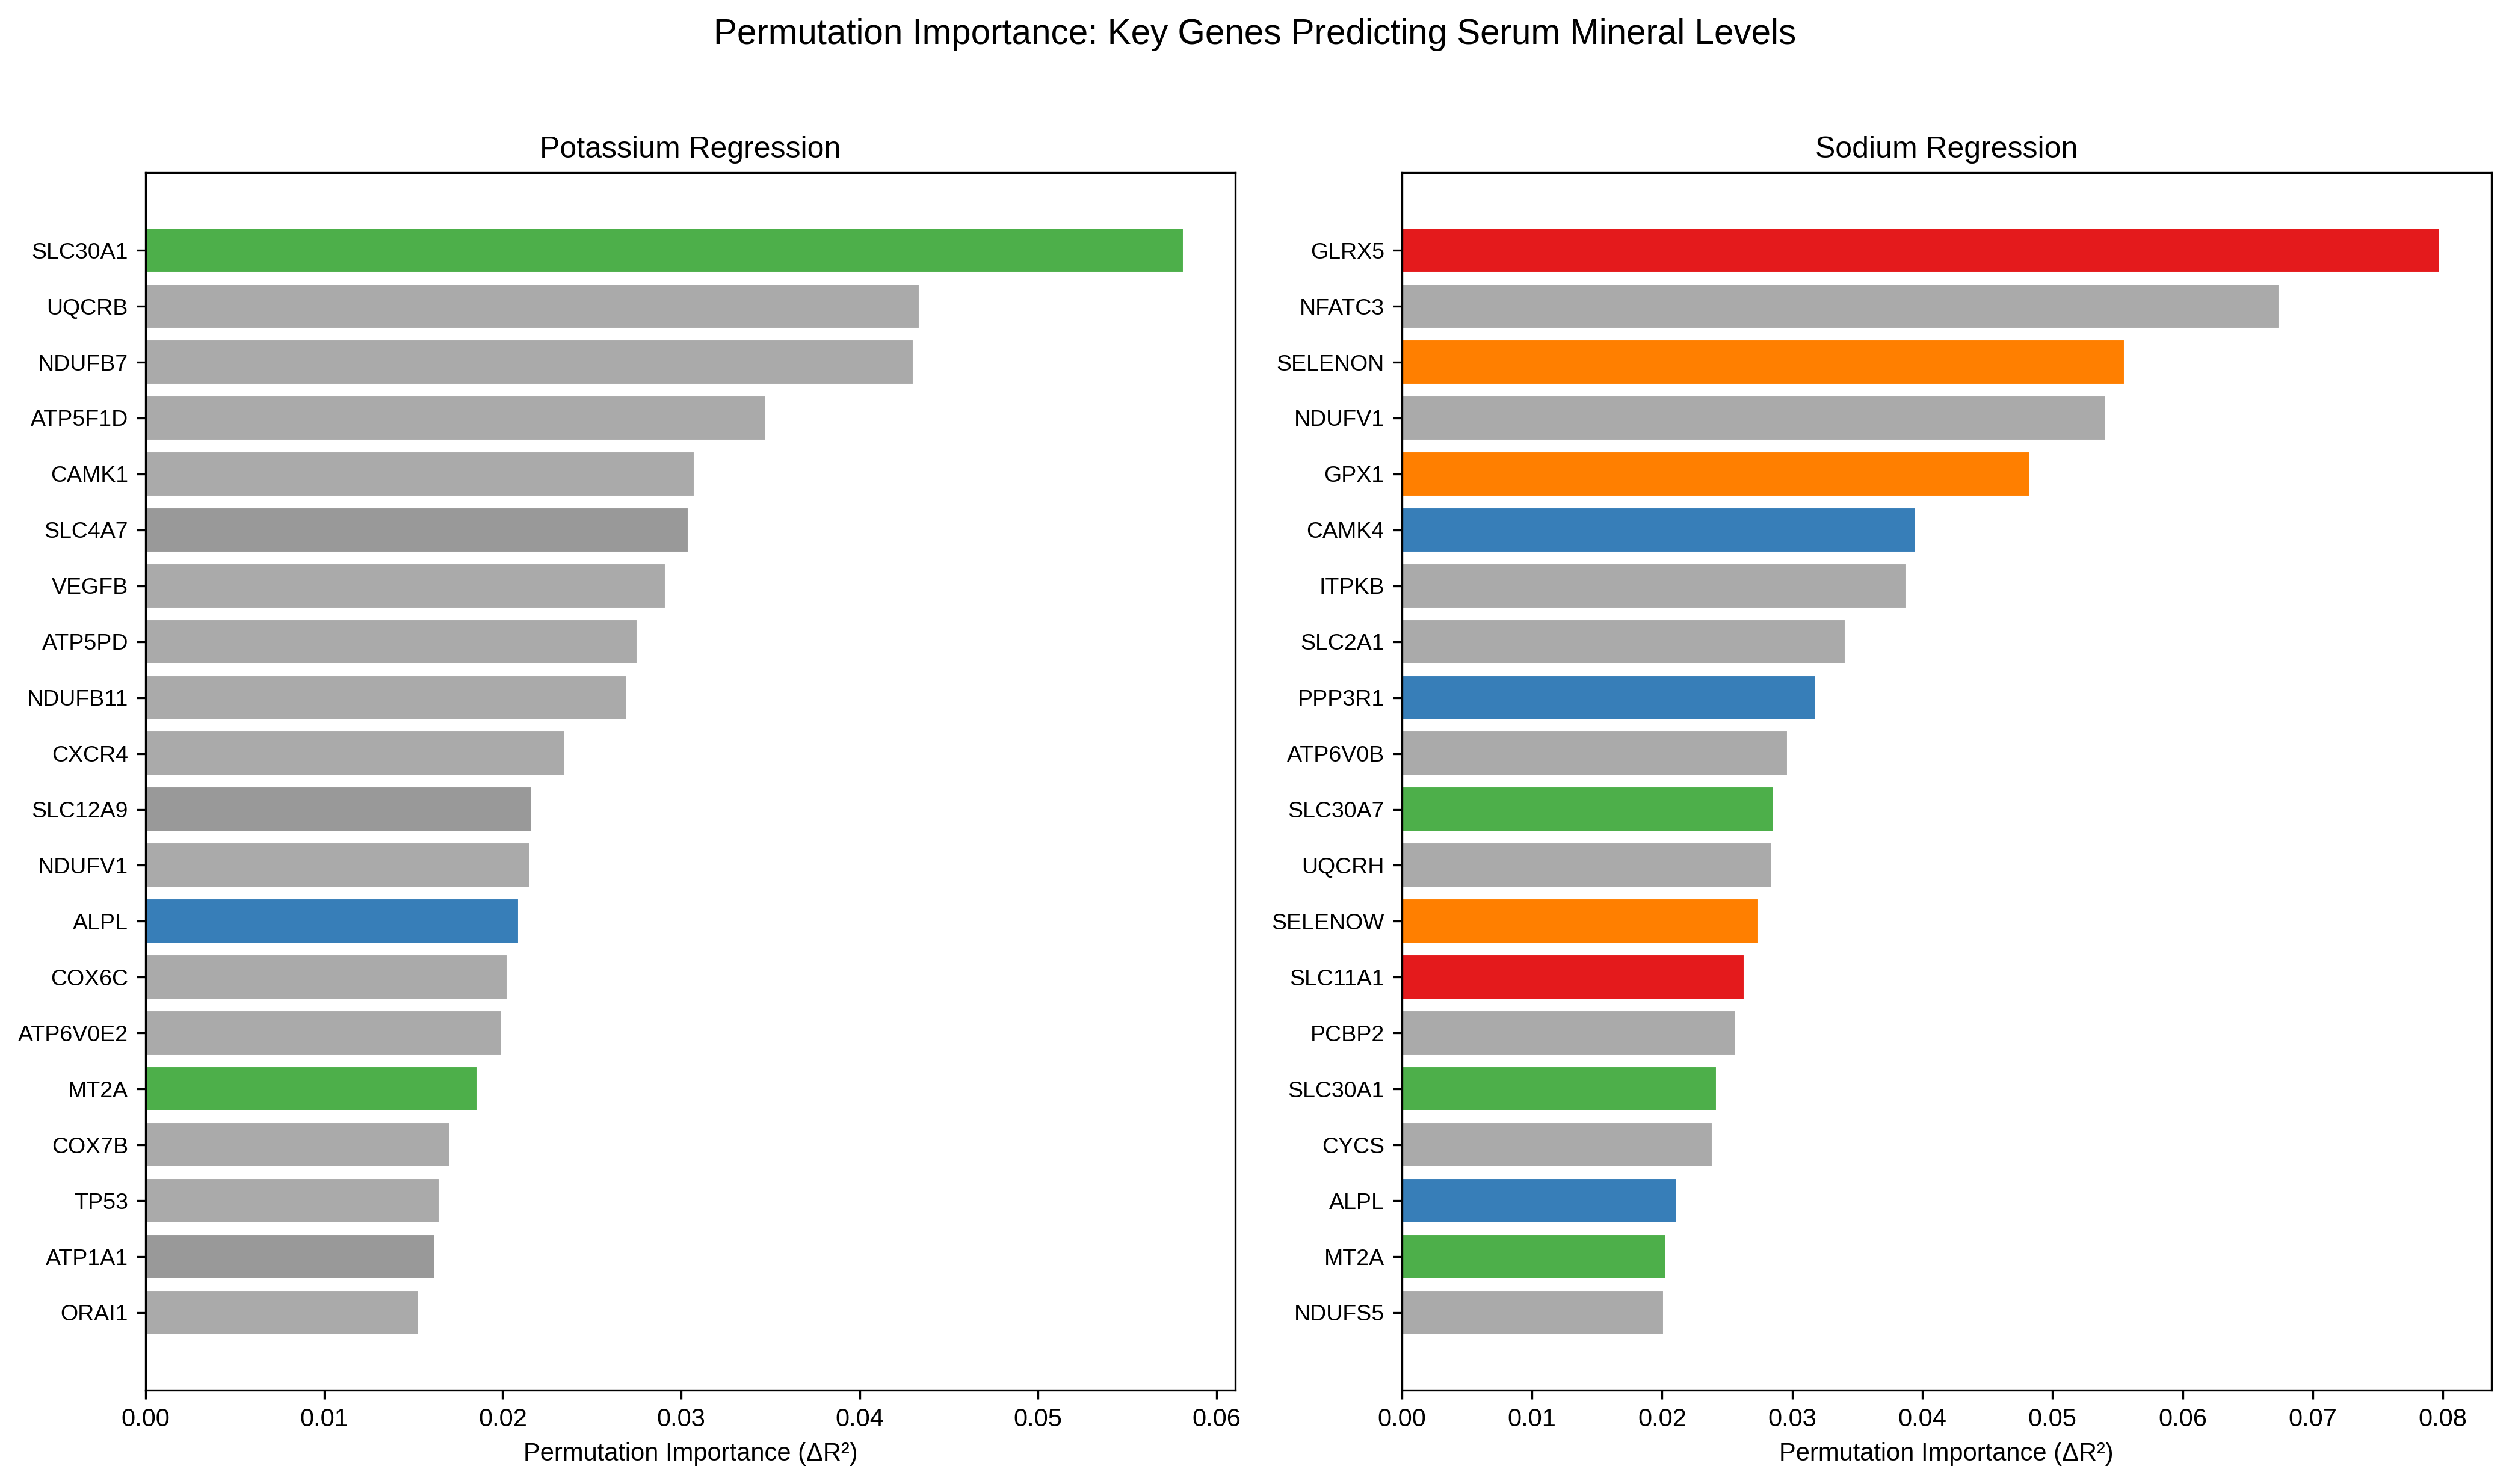
\includegraphics[width=\textwidth]{figures/fig3_barplot_importance.png}
\caption{Permutation importance for potassium (left) and sodium (right) regression. Bar colors indicate the primary mineral association of each gene. Genes from multiple mineral pathways contribute to predicting serum mineral levels.}
\label{fig:importance}
\end{figure}

\subsection{Cross-Species Concordance}

Rodent liver RNA-seq (OSD-47, FLT vs GC, $n=3$ per group) identified 365 genes with |log$_2$FC| $>$ 0.5 and $p$ $<$ 0.05 (relaxed threshold due to small sample size). After mapping mouse genes to human orthologs (13,825 genes mapped), 587 mineral-pathway genes were shared between species.

Directional concordance analysis revealed no significant agreement between astronaut peripheral blood and rodent liver mineral-pathway responses (Spearman $r$ = 0.007, $p$ = 0.87; binomial test $p$ = 1.0). Among the 41 astronaut DE genes with rodent orthologs, 51.2\% showed concordant directionality --- at chance level. Mineral-specific concordance ranged from 0\% (zinc, sodium, phosphorus, manganese) to 14\% (magnesium).

This lack of concordance likely reflects fundamental differences between the two datasets: (1) tissue specificity (astronaut peripheral blood vs rodent liver), (2) mission duration (3-day LEO vs 21-day ISS), (3) species differences (human vs mouse), and (4) radiation environment (LEO vs ISS altitude).

\begin{figure}[H]
\centering
\begin{subfigure}{0.48\textwidth}
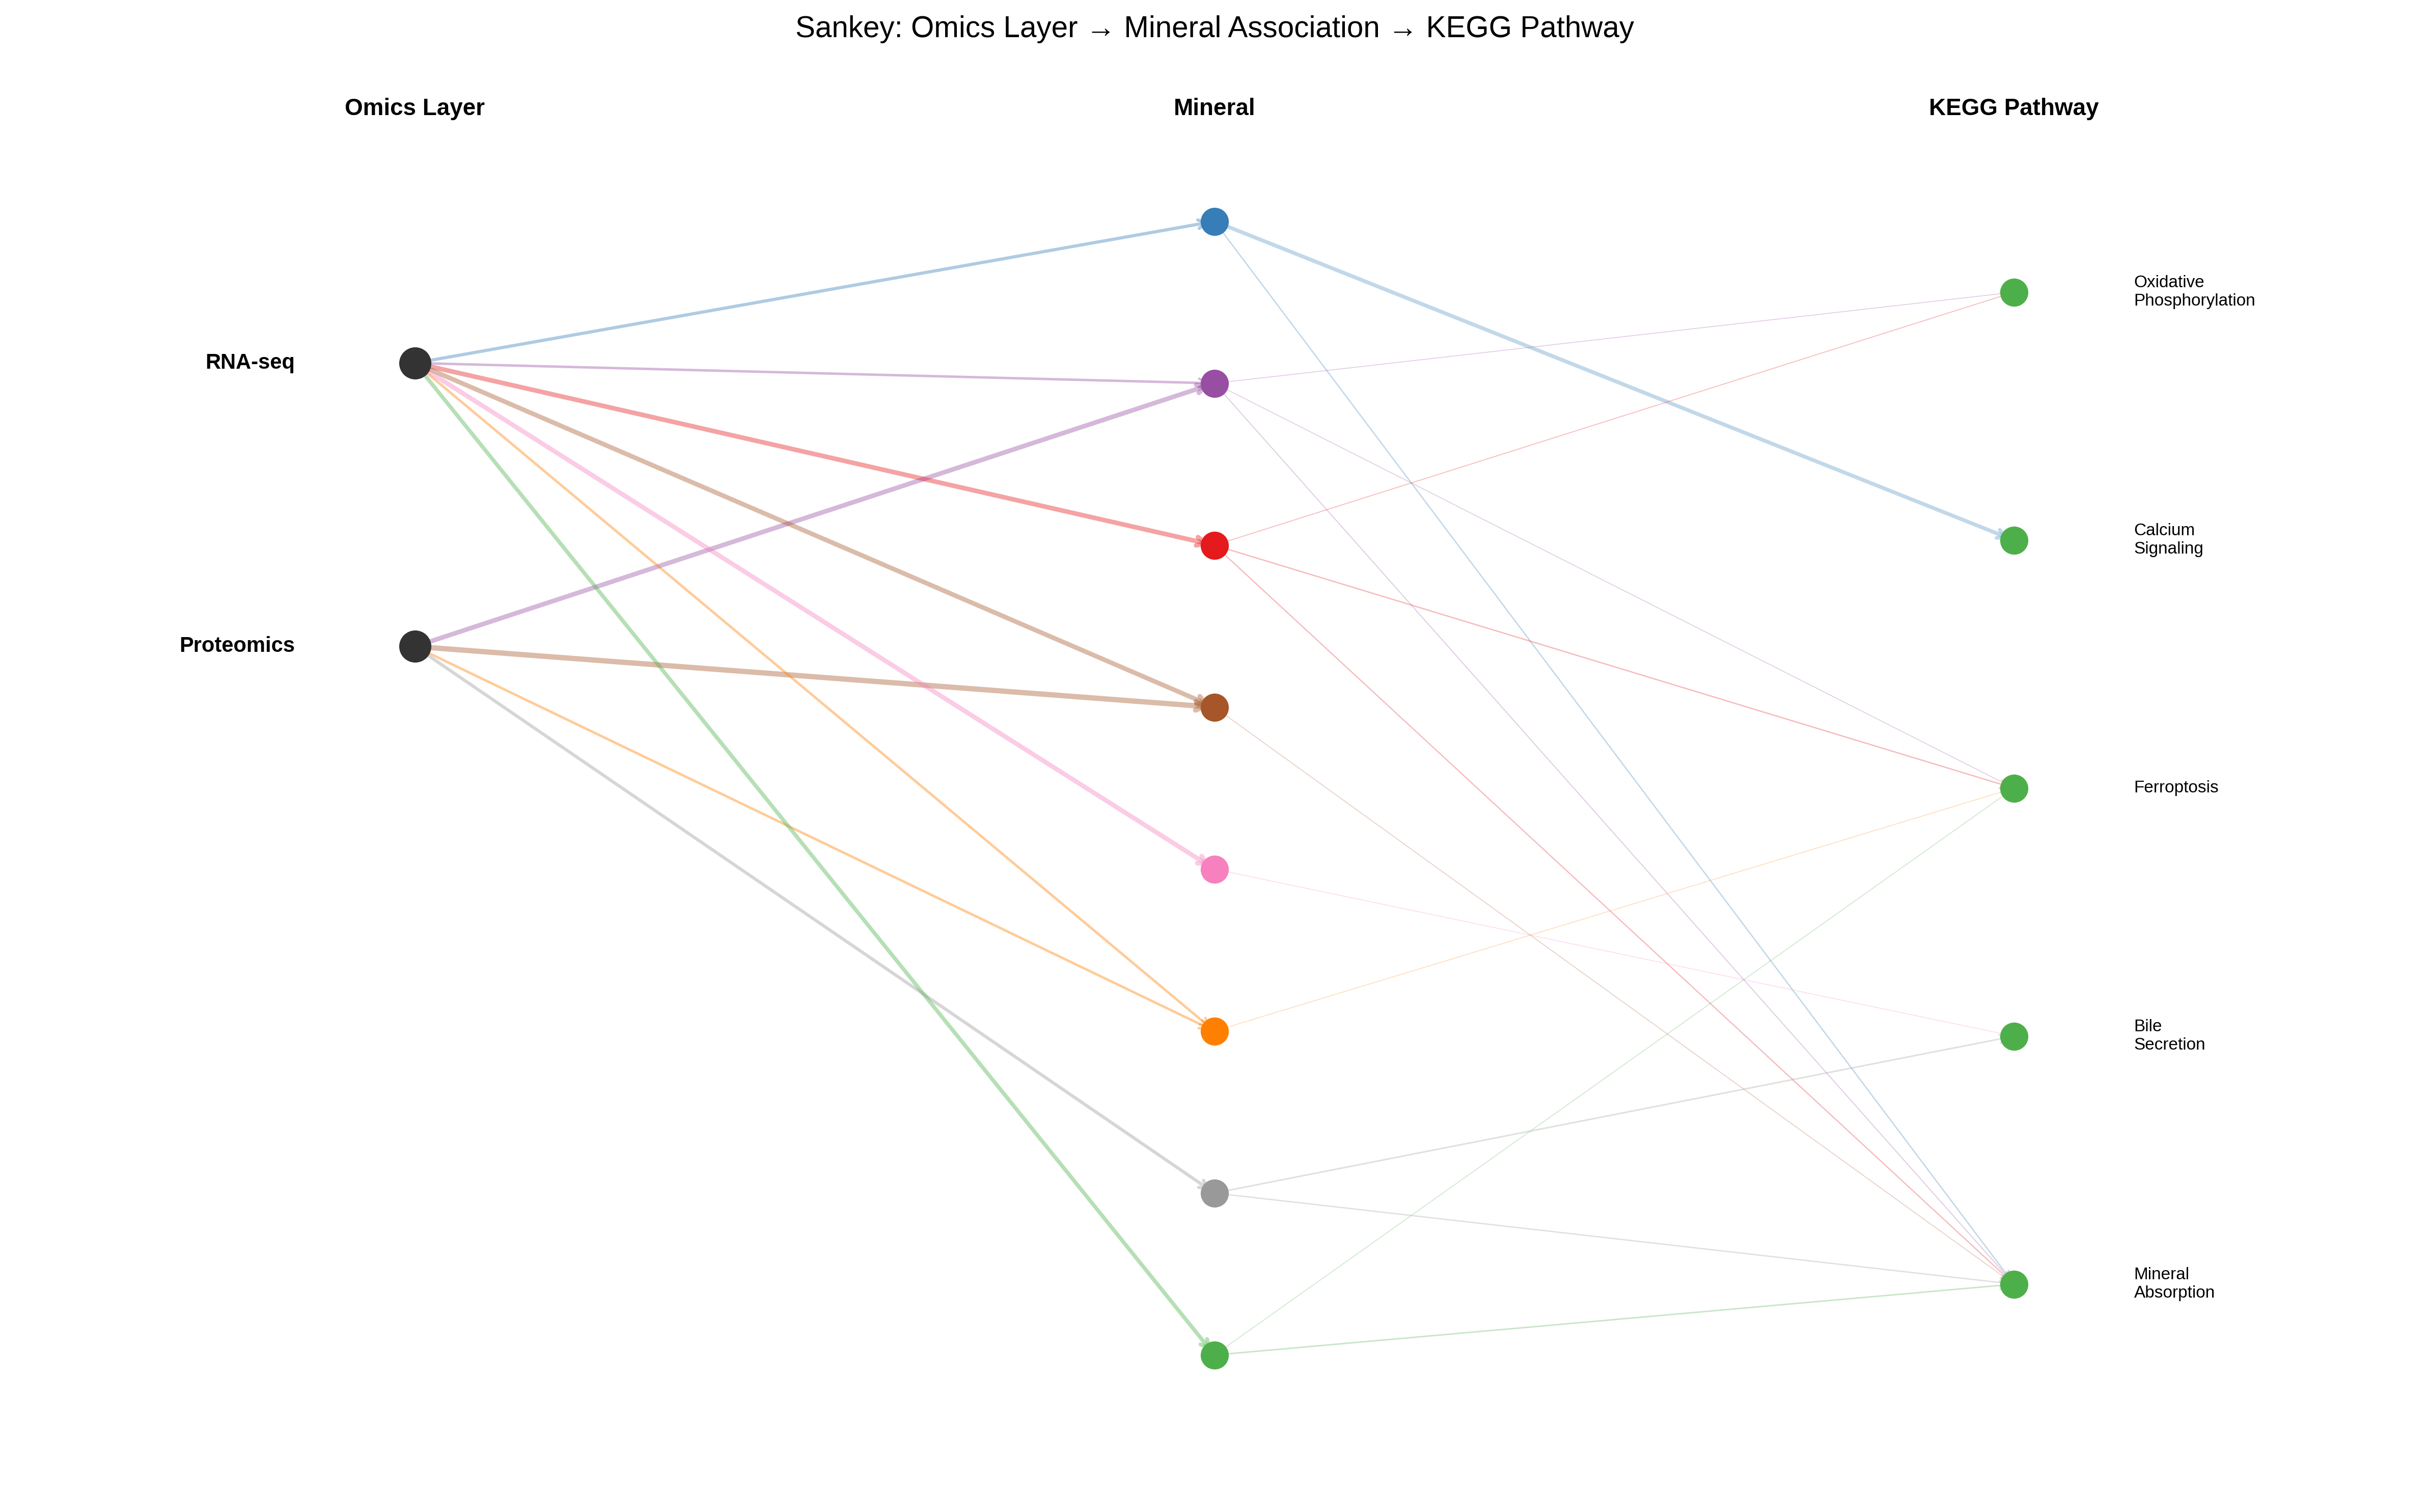
\includegraphics[width=\textwidth]{figures/fig4_sankey_omics_minerals.png}
\caption{}
\end{subfigure}
\hfill
\begin{subfigure}{0.48\textwidth}
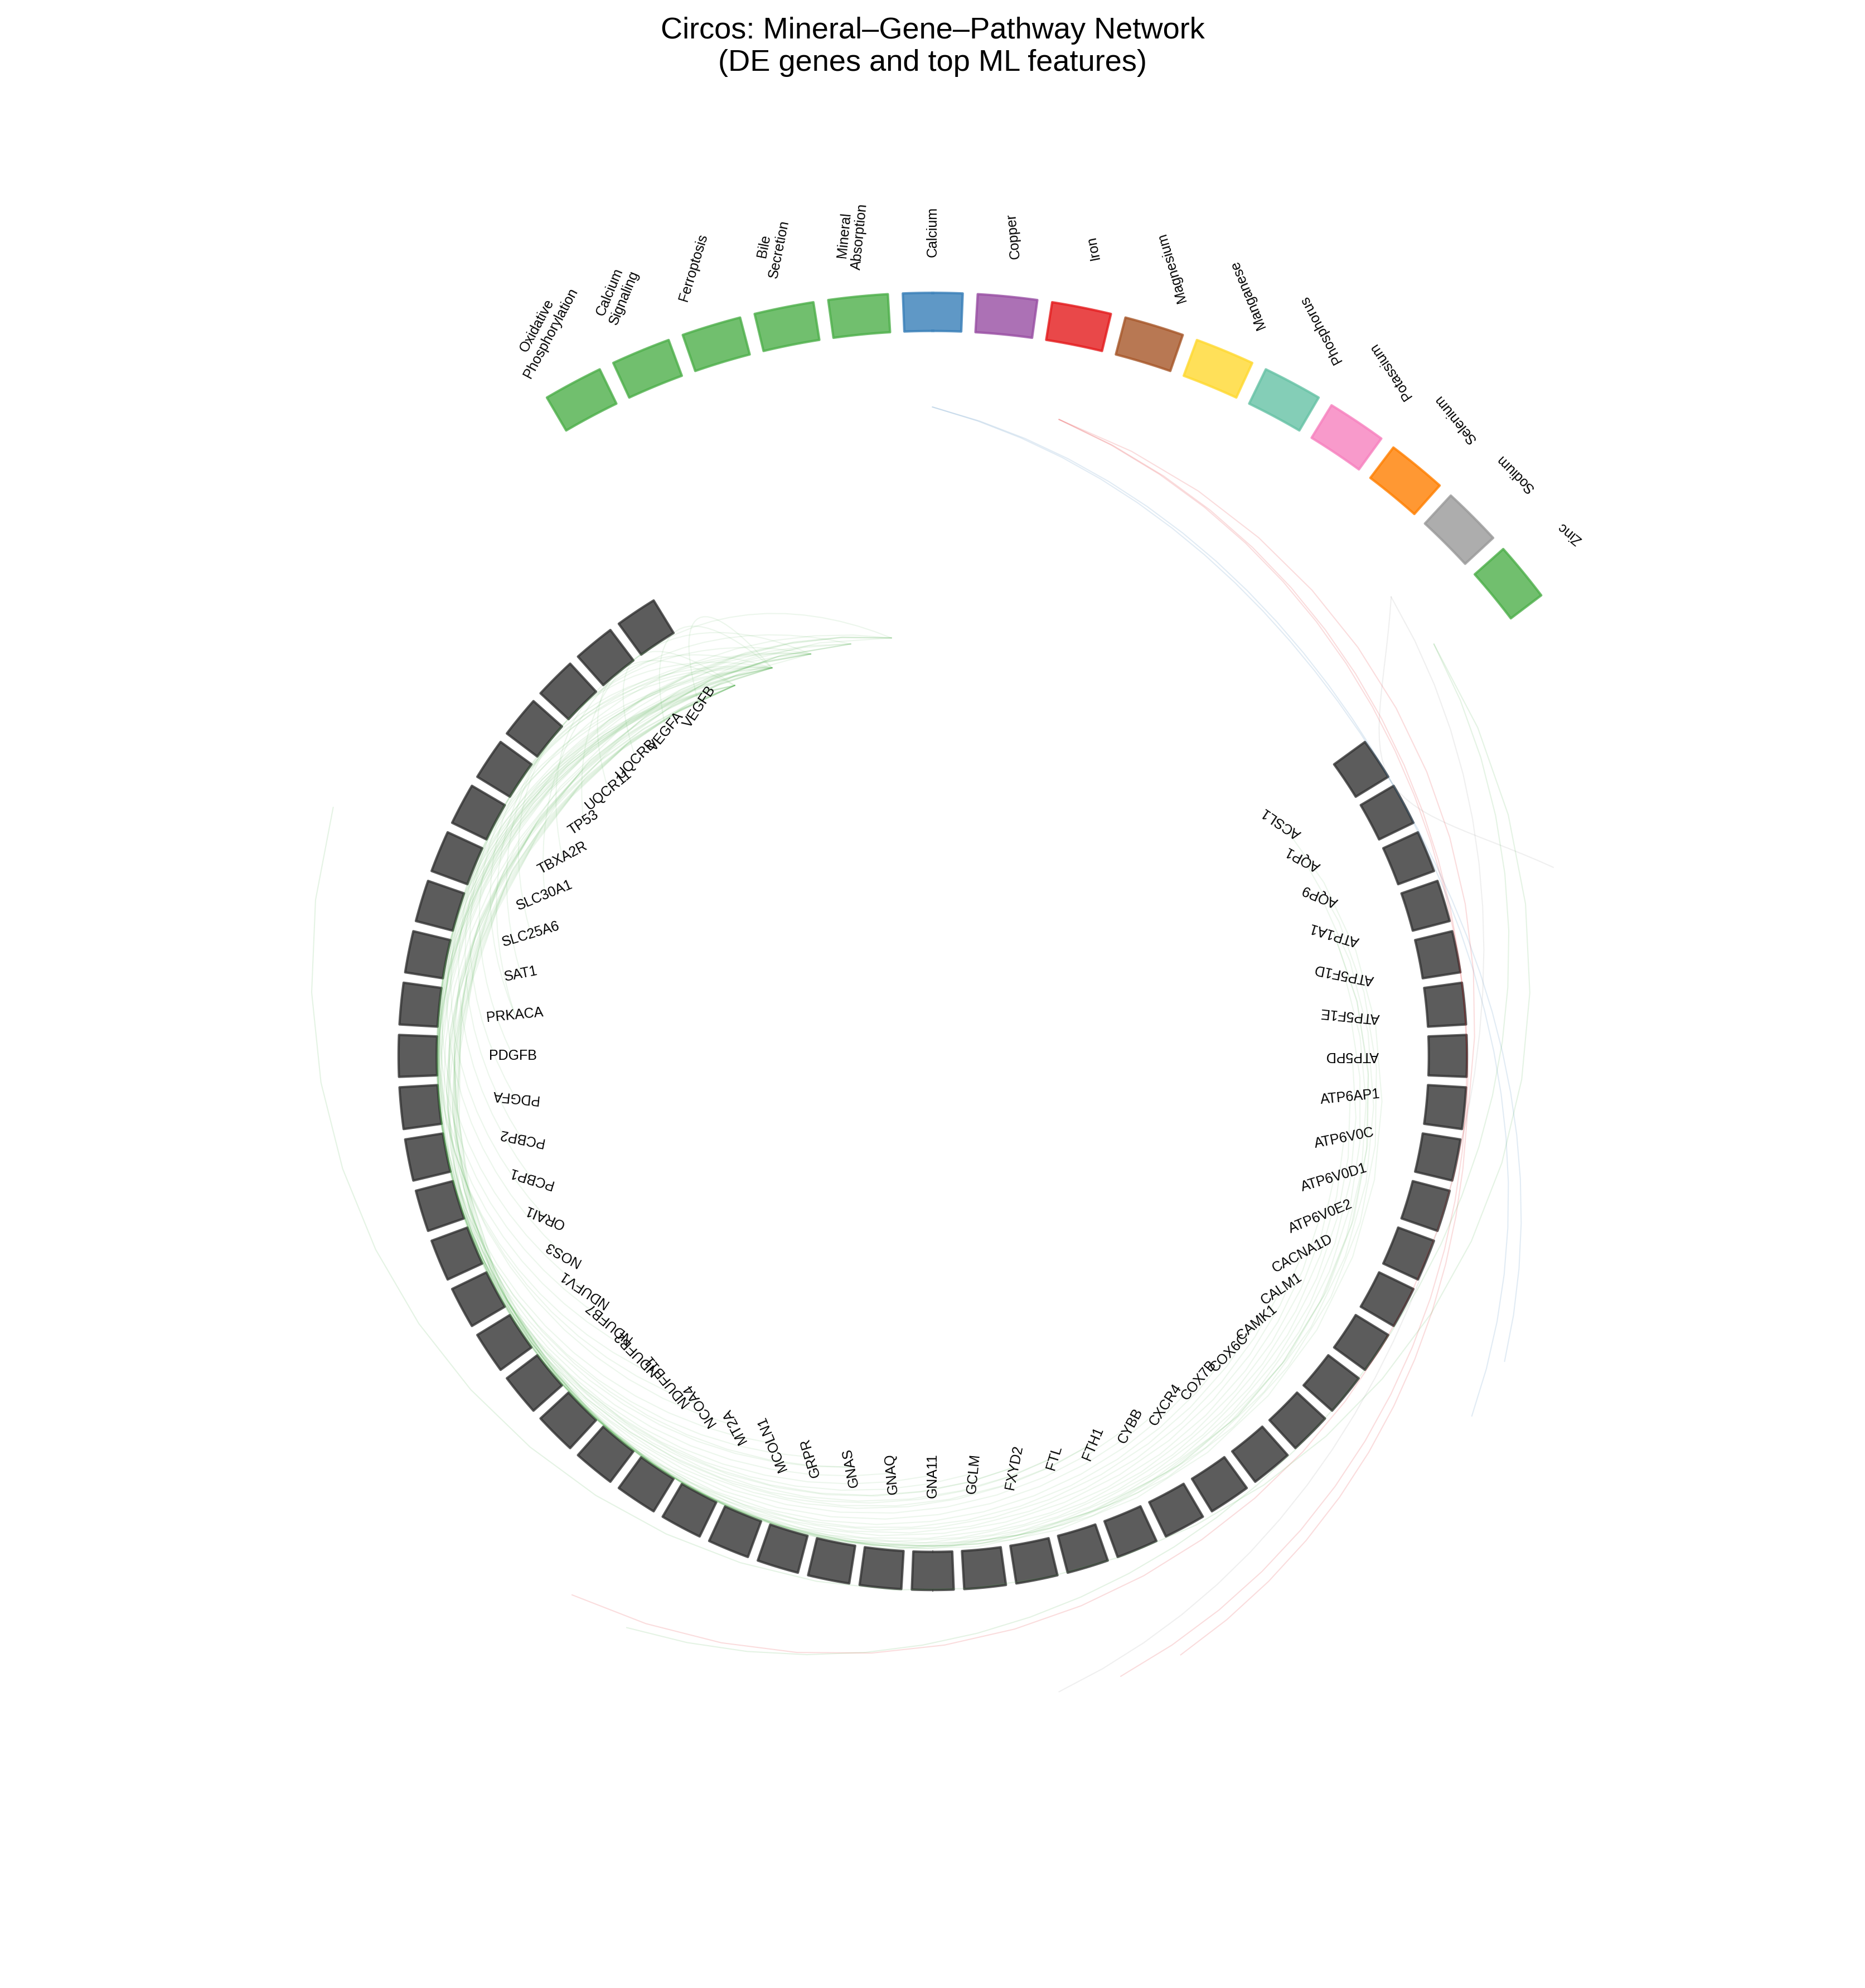
\includegraphics[width=\textwidth]{figures/fig5_circos_mineral_pathway.png}
\caption{}
\end{subfigure}
\caption{(a) Sankey diagram showing the flow from omics layer (RNA-seq, proteomics) through mineral associations to KEGG pathways. (b) Circos plot of mineral--gene--pathway connections, highlighting differentially expressed genes and top ML features.}
\label{fig:sankey_circos}
\end{figure}

\subsection{Systems Biology Atlas}

The systems biology atlas (Figure~\ref{fig:atlas}) integrates five panels: (A) KEGG pathway expression changes across flight comparisons, (B) mineral-pathway gene set sizes, (C) up/down-regulated DE genes per mineral, (D) cross-species concordance scatter plot, and (E) top 25 mineral-pathway DE genes. The atlas reveals that copper and magnesium pathways show the most consistent dysregulation across omics layers, while calcium signaling genes show the largest individual fold changes.

\begin{figure}[H]
\centering
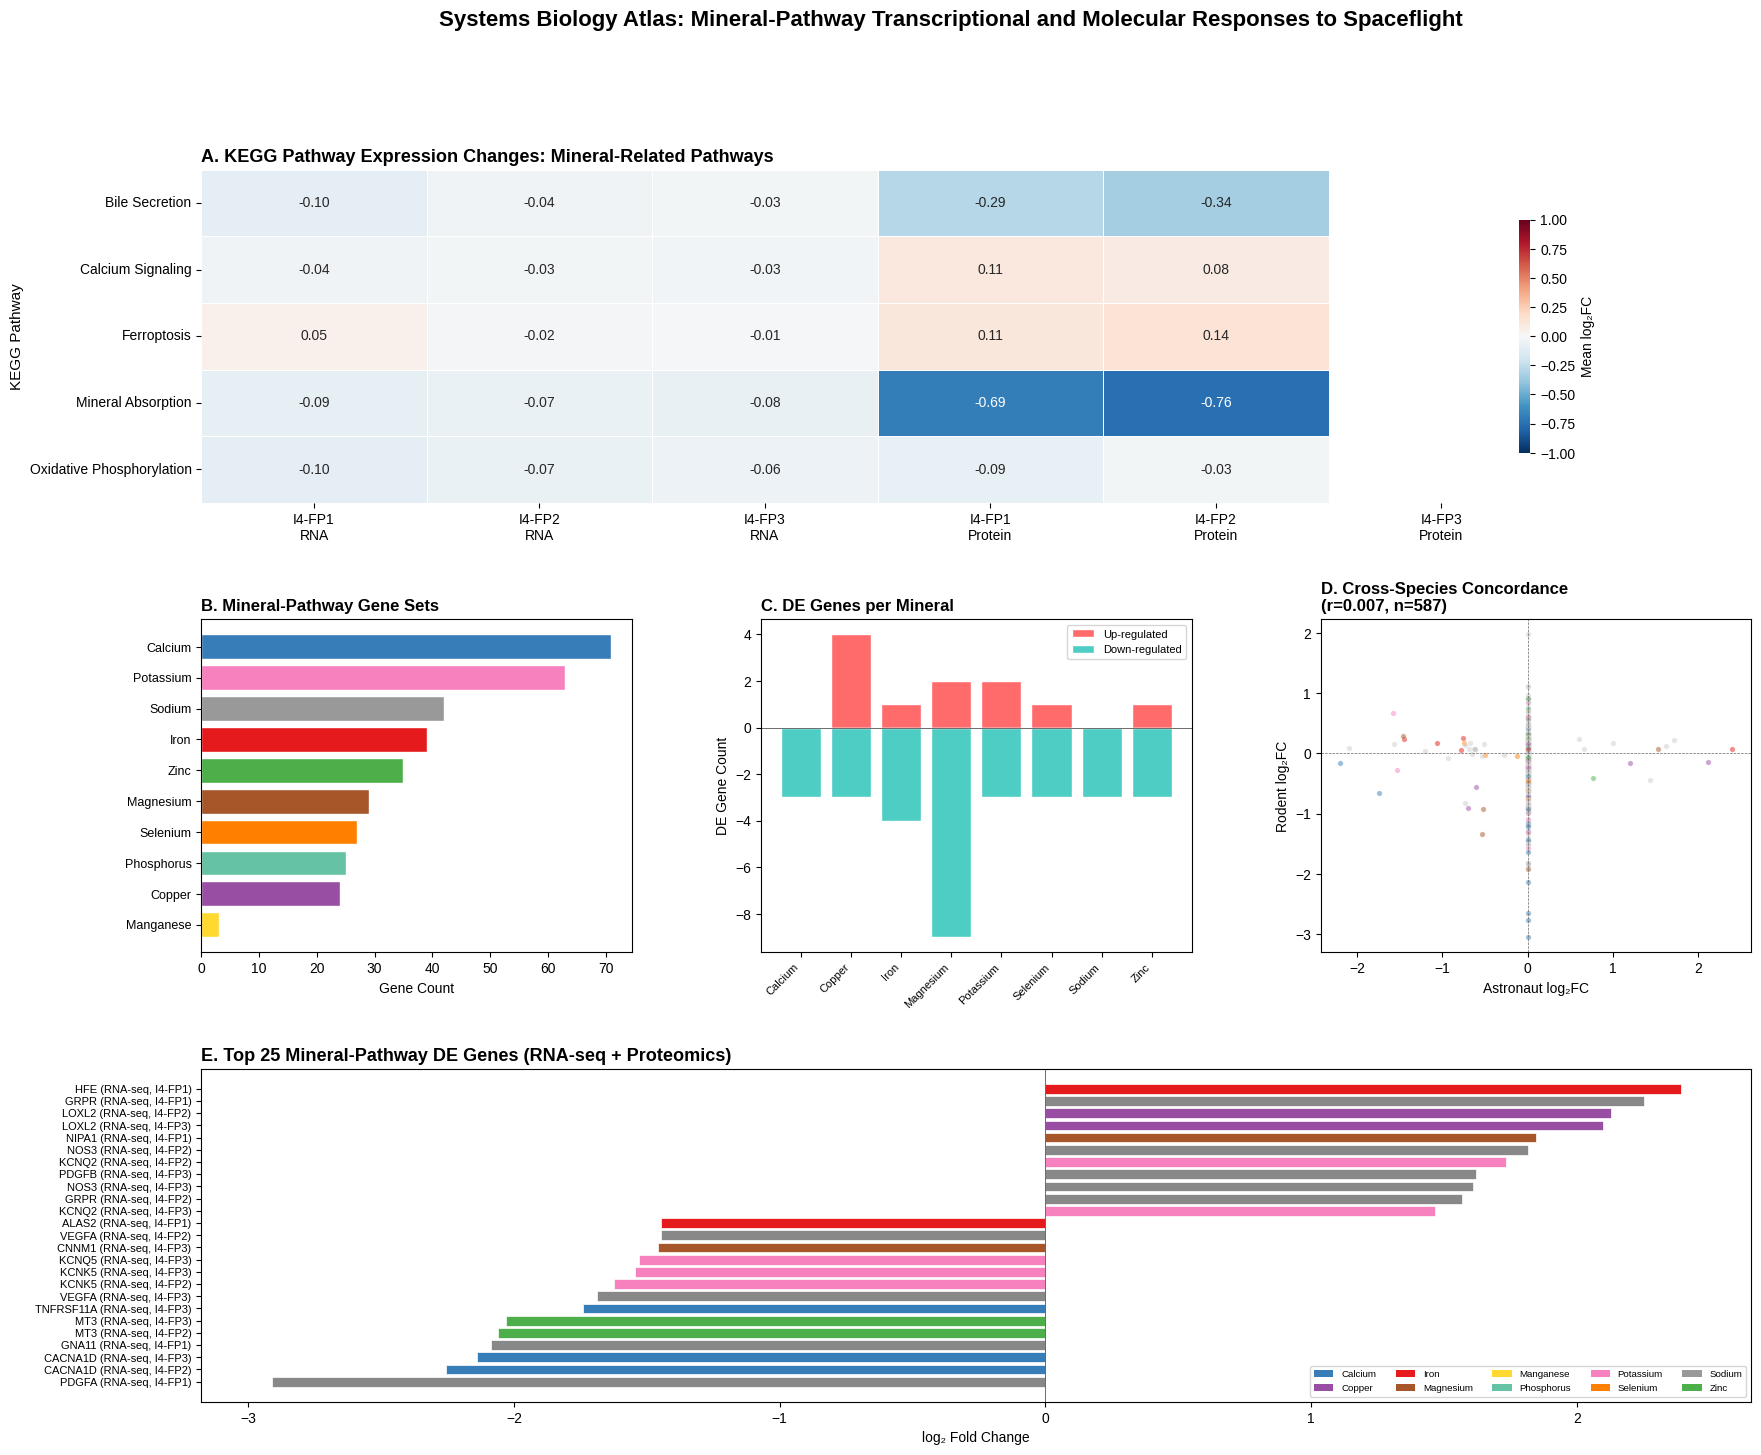
\includegraphics[width=\textwidth]{figures/fig8_systems_biology_atlas.png}
\caption{Systems biology atlas. (A) KEGG pathway mean log$_2$FC across comparisons (RNA-seq and proteomics). (B) Gene counts per mineral gene set. (C) Up/down-regulated DE genes per mineral. (D) Cross-species concordance scatter (astronaut vs rodent log$_2$FC). (E) Top 25 mineral-pathway DE genes with mineral color coding.}
\label{fig:atlas}
\end{figure}

\begin{figure}[H]
\centering
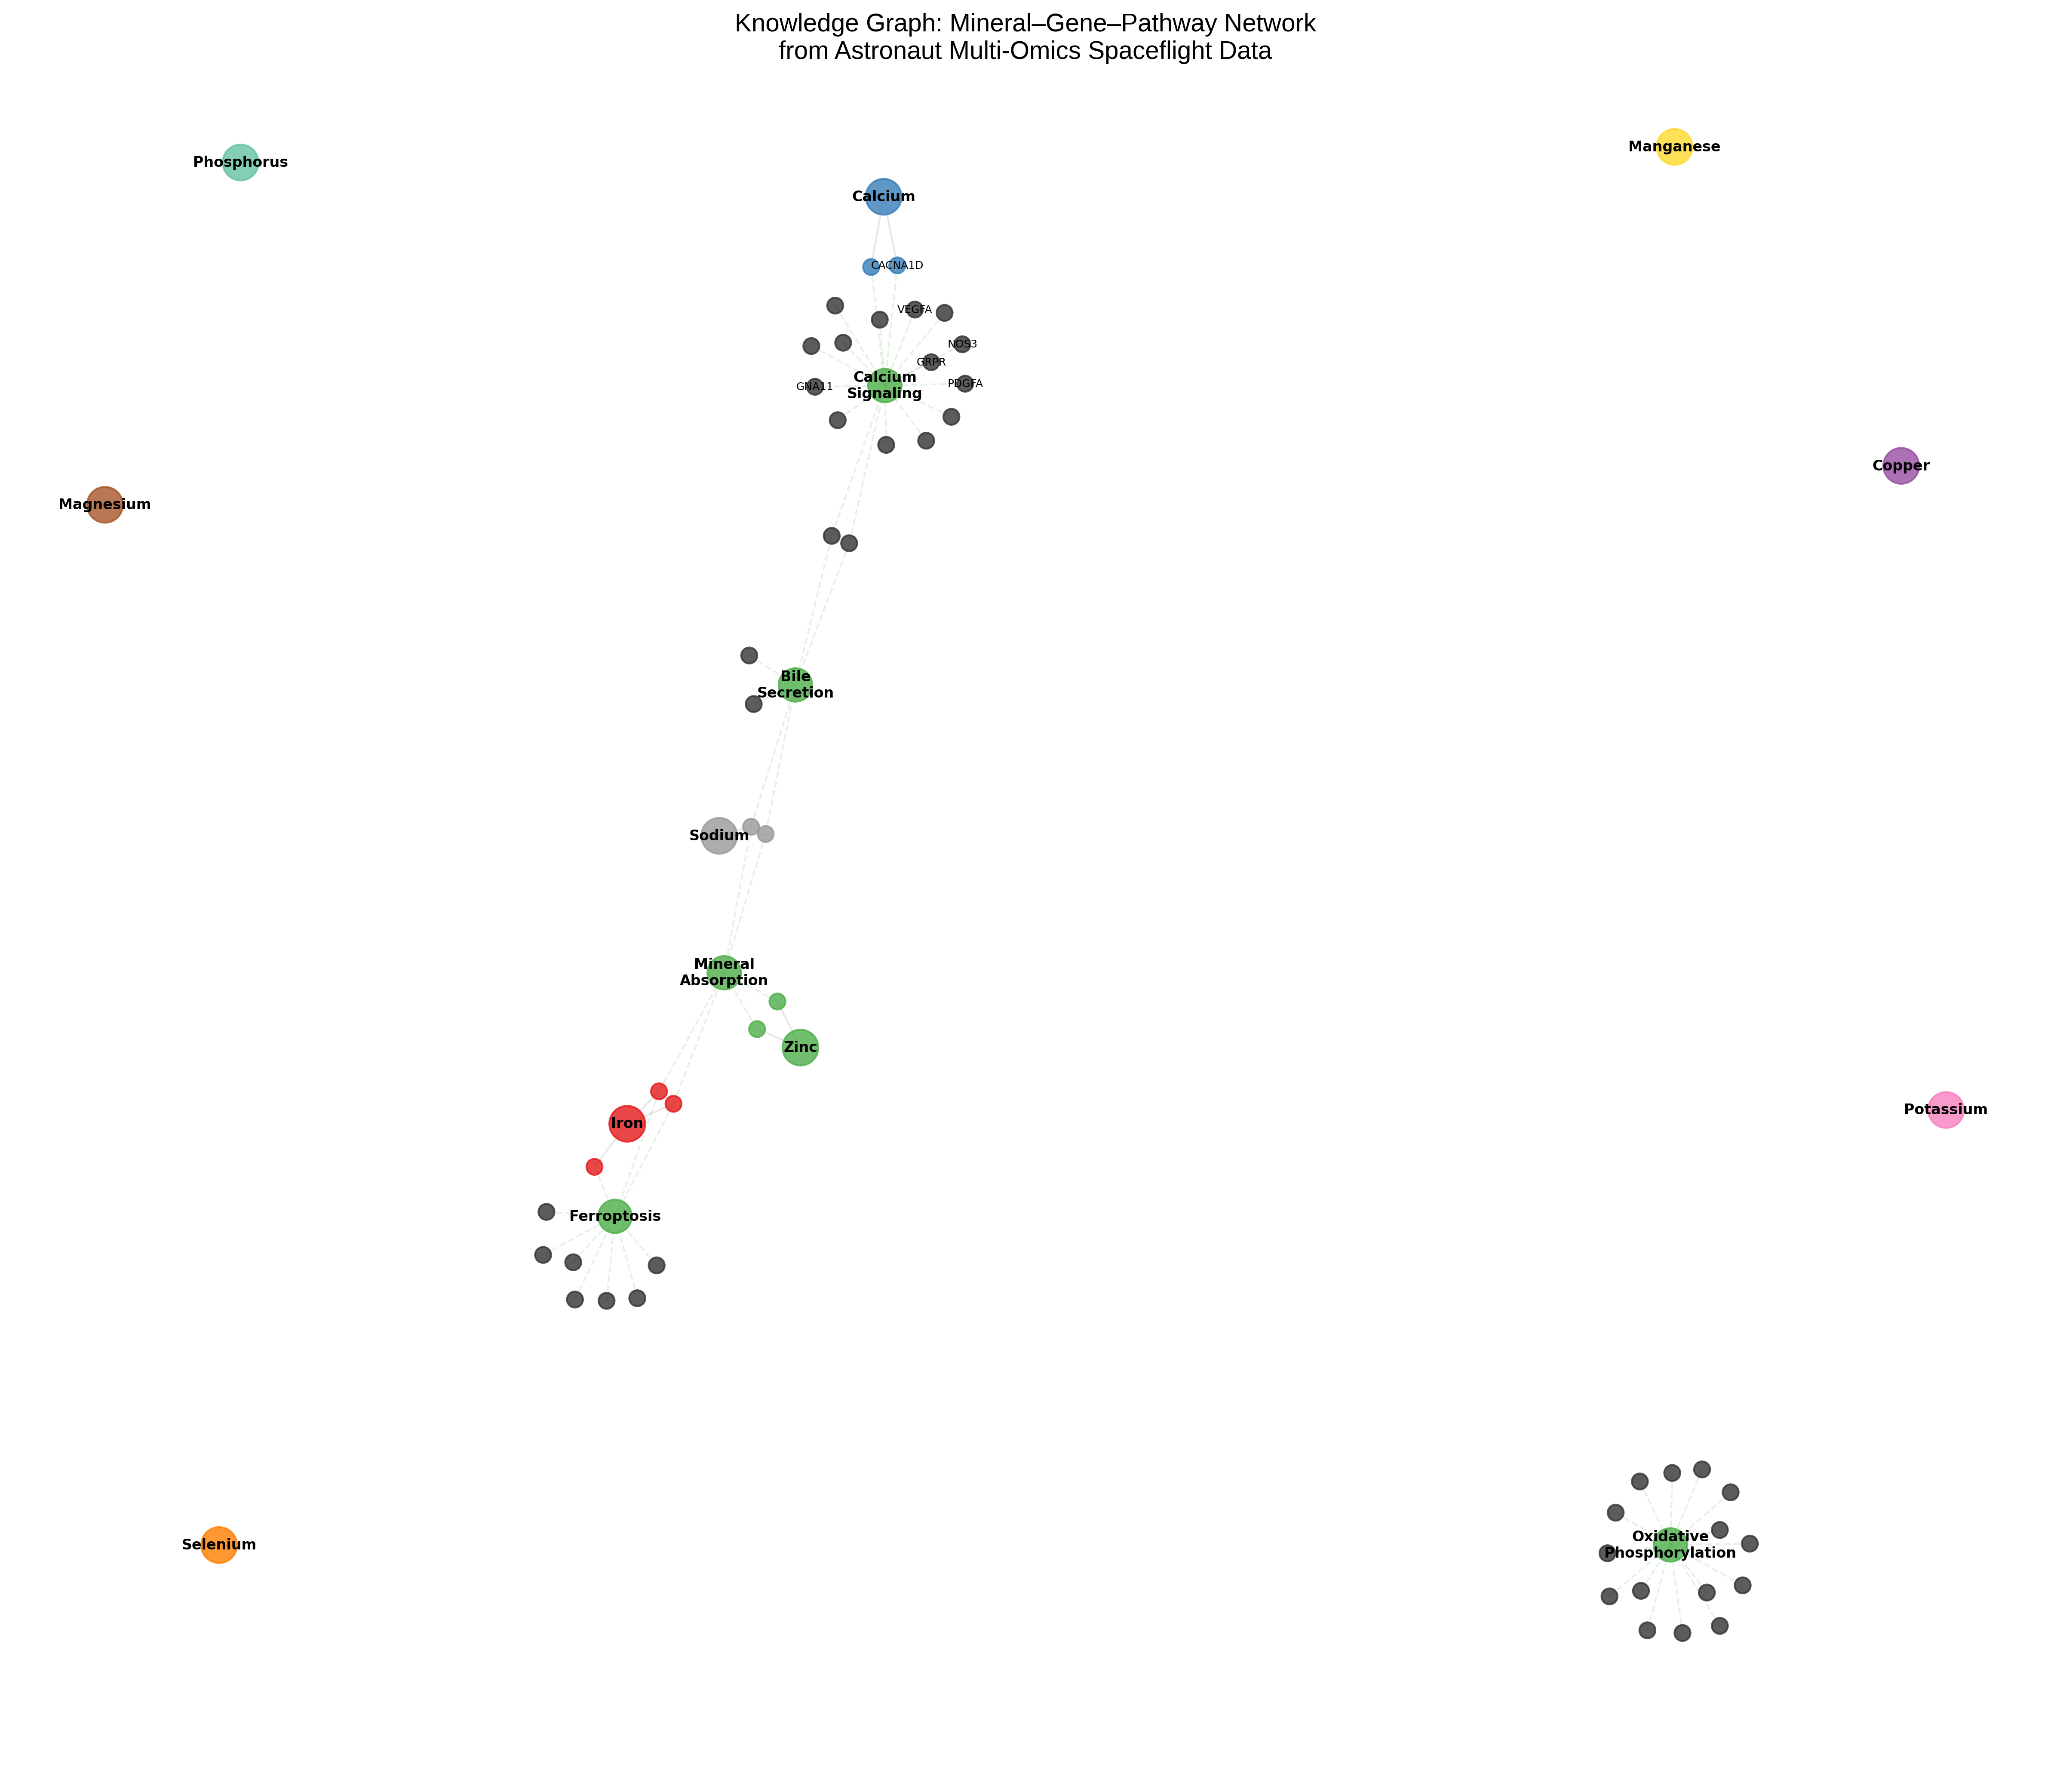
\includegraphics[width=\textwidth]{figures/fig6_knowledge_graph.png}
\caption{Knowledge graph of the mineral--gene--pathway network. Mineral nodes (colored circles) connect to gene nodes (small circles) and KEGG pathway nodes (green). Edges represent mineral-gene associations (solid grey) and gene-pathway memberships (dashed green). Top DE genes are labeled.}
\label{fig:knowledge_graph}
\end{figure}

% ════════════════════════════════════════════════════════════════════
% DISCUSSION
% ════════════════════════════════════════════════════════════════════
\section{Discussion}

This study presents the first systematic multi-omics analysis of mineral-pathway transcriptional and molecular responses to spaceflight, integrating astronaut data from the Inspiration4 mission with rodent data from NASA's Rodent Research program. Our findings reveal that spaceflight alters the expression of genes involved in copper, magnesium, calcium, and potassium homeostasis, and that mineral-pathway gene expression carries predictive information about serum mineral levels.

\subsection{Copper Pathway Dysregulation}

The most consistent mineral-pathway finding was copper-related gene dysregulation. In proteomics, APP (amyloid precursor protein, a copper-binding protein) was up-regulated in both I4-FP1 and I4-FP2, while LOX and LOXL1 (copper-dependent lysyl oxidases) were down-regulated. In RNA-seq, LOXL2 was up-regulated in I4-FP3. Lysyl oxidases are copper-dependent enzymes critical for collagen cross-linking and connective tissue integrity \citep{smithmungo1998}. Their down-regulation may reflect altered copper availability or a protective response to microgravity-induced connective tissue changes. The up-regulation of APP, which binds copper with high affinity, may represent a compensatory response to maintain copper homeostasis.

\subsection{Magnesium-Binding S100 Proteins}

The S100 family of magnesium-binding proteins (S100A8, S100A9, S100A12) showed consistent down-regulation in proteomics. S100A8/A9 form the calprotectin heterodimer, which plays roles in innate immunity and inflammation \citep{wang2018}. Their suppression may reflect the anti-inflammatory environment of microgravity or altered magnesium availability. Magnesium is a cofactor for over 300 enzymes, and S100 proteins require magnesium for their structural integrity and function.

\subsection{Calcium and Potassium Channels}

The down-regulation of CACNA1D (voltage-gated calcium channel, log$_2$FC = $-$2.14) represents one of the largest fold changes observed. This may reflect a cellular adaptation to microgravity-induced calcium flux, as mechanical unloading alters mechanotransduction signalling in bone cells \citep{hughesfulford2004}. The up-regulation of KCNQ2 (potassium channel) is consistent with the post-flight decline in serum potassium observed in three of four astronauts, potentially reflecting compensatory transcriptional up-regulation in response to hypokalemia.

\subsection{Machine Learning Predictions}

The regression analysis demonstrated that mineral-pathway gene expression predicts serum potassium ($r$ = 0.50) and sodium ($r$ = 0.46) levels, despite the extremely small sample size ($n=16$, LOO-CV). This suggests that the transcriptomic signature of mineral homeostasis genes captures physiologically meaningful variation in serum mineral status. The permutation importance analysis revealed that genes from multiple mineral pathways (calcium, zinc, selenium, iron) contribute to predicting potassium and sodium levels, highlighting the interconnectedness of mineral homeostasis systems.

\subsection{Cross-Species Differences}

The absence of cross-species concordance ($r$ = 0.007) between astronaut peripheral blood and rodent liver is an important negative finding. This likely reflects the fundamental biological differences between the two experimental systems: different tissues (blood vs liver), different mission durations (3 days vs 21 days), different species (human vs mouse), and different spaceflight environments (LEO vs ISS). These results caution against direct extrapolation of rodent mineral-pathway findings to human spaceflight and underscore the need for human-specific data.

\subsection{Limitations}

Several limitations should be noted. First, the sample size is extremely small ($n=4$ astronauts, $n=3$ rodents per group), limiting statistical power. Second, only five minerals were directly measured in serum (Ca, K, Na, Cl, CO$_2$); other minerals (Fe, Mg, Zn, Cu, Se, P, Mn) were assessed only through pathway-level transcriptomic evidence. Third, the DESeq2 method yielded uniformly near-zero log$_2$FC values, and we relied on the pipeline-transcriptome-de method for meaningful fold changes. Fourth, TabPFN, the intended ML approach, could not be used due to license-gated model weights; sklearn models were used instead. Fifth, the cross-species comparison is confounded by tissue and mission duration differences. Sixth, pathview could not be installed due to Rgraphviz dependency issues; a custom Python-based atlas was created instead.

\subsection{Future Directions}

Future studies should: (1) incorporate data from longer-duration missions (ISS, Artemis) to assess chronic mineral-pathway adaptation; (2) directly measure a broader panel of minerals (Fe, Mg, Zn, Cu, Se) in astronaut serum; (3) use single-cell RNA-seq to resolve cell-type-specific mineral-pathway responses; (4) apply TabPFN or other foundation models when larger datasets become available; and (5) match tissues between species for more valid cross-species comparisons.

% ════════════════════════════════════════════════════════════════════
% CONCLUSION
% ════════════════════════════════════════════════════════════════════
\section{Conclusion}

This study demonstrates that spaceflight alters the expression of mineral homeostasis genes, with copper-dependent enzymes, magnesium-binding S100 proteins, and calcium/potassium channels showing the most consistent dysregulation. Mineral-pathway gene expression predicts serum potassium and sodium levels, suggesting that transcriptomic signatures of mineral homeostasis carry physiologically meaningful information. The lack of cross-species concordance between astronaut blood and rodent liver highlights the need for human-specific data in spaceflight mineral research. These findings provide a foundation for developing mineral-status biomarkers and nutritional countermeasures for long-duration spaceflight.

% ════════════════════════════════════════════════════════════════════
% REFERENCES
% ════════════════════════════════════════════════════════════════════
\section*{References}

\begin{thebibliography}{99}

\bibitem[Williams(2009)]{williams2009}
Williams D, Kuipers A, Mukai C, Thirsk R. Acclimation during space flight: effects on human physiology. \textit{CMAJ}. 2009;180(13):1317--1323. doi:10.1503/cmaj.090628

\bibitem[Smith et al.(2005)]{smith2005}
Smith SM, Wastney ME, O'Brien KO, et al. Bone markers, calcium metabolism, and calcium kinetics during extended-duration space flight on the Mir space station. \textit{J Bone Miner Res}. 2005;20(2):208--218. doi:10.1359/JBMR.041105

\bibitem[Norsk et al.(2015)]{norsk2015}
Norsk P, Asmar A, Damgaard M, Christensen NJ. Fluid shifts, vasodilatation and ambulatory blood pressure reduction during long duration spaceflight. \textit{J Physiol}. 2015;593(3):573--584. doi:10.1113/jphysiol.2014.284869

\bibitem[Stein(2002)]{stein2002}
Stein TP. Space flight and oxidative stress. \textit{Nutrition}. 2002;18(10):867--871. doi:10.1016/S0899-9007(02)00938-3

\bibitem[Overbey et al.(2024)]{overbey2024}
Overbey EG, Kim J, Tierney BT, et al. The Space Omics and Medical Atlas (SOMA) and international astronaut biobank. \textit{Nature}. 2024;632(8027):1145--1154. doi:10.1038/s41586-024-07639-y

\bibitem[Smith et al.(2015)]{smith2015}
Smith SM, Heer M, Shackelford LC, et al. Bone metabolism and renal stone risk during International Space Station missions. \textit{Bone}. 2015;81:712--720. doi:10.1016/j.bone.2015.10.002

\bibitem[Smith(2002)]{smith2002iron}
Smith SM. Red blood cell and iron metabolism during space flight. \textit{Nutrition}. 2002;18(10):864--866. doi:10.1016/S0899-9007(02)00912-7

\bibitem[Smith-Mungo and Kagan(1998)]{smithmungo1998}
Smith-Mungo LI, Kagan HM. Lysyl oxidase: properties, regulation and multiple functions in biology. \textit{Matrix Biol}. 1998;16(7):387--398. doi:10.1016/S0945-053X(98)90012-9

\bibitem[Wang et al.(2018)]{wang2018}
Wang S, Song R, Wang Z, et al. S100A8/A9 in inflammation. \textit{Front Immunol}. 2018;9:1298. doi:10.3389/fimmu.2018.01298

\bibitem[Hughes-Fulford(2004)]{hughesfulford2004}
Hughes-Fulford M. Signal transduction and mechanical stress. \textit{Sci STKE}. 2004;2004(249):re12. doi:10.1126/stke.2492004re12

\end{thebibliography}

\end{document}
